\chapter{Red-Black Trees}
\chaplabel{redblack}

\index{binary search tree!red-black}%
\index{red-black tree}%
In this chapter, we present red-black trees, a version of binary search
trees with logarithmic height.  Red-black trees are one of the most
widely used data structures.  They appear as the primary search structure
in many library implementations, including the Java Collections Framework
and several implementations of the C++ Standard Template Library. They
are also used within the Linux operating system kernel.  There are
several reasons for the popularity of red-black trees:
\begin{enumerate}
\item A red-black tree storing #n# values has height at most $2\log #n#$.
\item The #add(x)# and #remove(x)# operations on a red-black tree run
   in $O(\log #n#)$ \emph{worst-case} time.
\item The amortized number of rotations performed during an #add(x)#
   or #remove(x)# operation is constant.
\end{enumerate}
The first two of these properties already put red-black trees 
ahead of skiplists, treaps, and scapegoat trees.
Skiplists and treaps rely on randomization and their $O(\log #n#)$
running times are only expected. Scapegoat trees have a guaranteed
bound on their height, but #add(x)# and #remove(x)# only run in $O(\log
#n#)$ amortized time.  The third property is just icing on the cake. It
tells us that  that the time needed to add or remove an element #x# is
dwarfed by the time it takes to find #x#.\footnote{Note that skiplists and
treaps also have this property in the expected sense. See
Exercises~\ref{exc:skiplist-changes} and \ref{exc:treap-rotates}.}

However, the nice properties of red-black trees come with a price:
implementation complexity. Maintaining a bound of $2\log #n#$ on the
height is not easy. It requires a careful analysis of a number of cases.
We must ensure that the implementation does exactly the right
thing in each case.  One misplaced rotation or change of colour produces
a bug that can be very difficult to understand and track down.

Rather than jumping directly into the implementation of red-black trees,
we will first provide some background on a related data structure:
2-4 trees.  This will give some insight into how red-black trees were
discovered and why efficiently maintaining them is even possible.

\section{2-4 Trees}
\seclabel{twofour}

A 2-4 tree is a rooted tree with the following properties:
\begin{prp}[height]
  All leaves have the same depth.
\end{prp}
\begin{prp}[degree]
  Every internal node has 2, 3, or 4 children.
\end{prp}
An example of a 2-4 tree is shown in \figref{twofour-example}.
\begin{figure}
  \begin{center}
    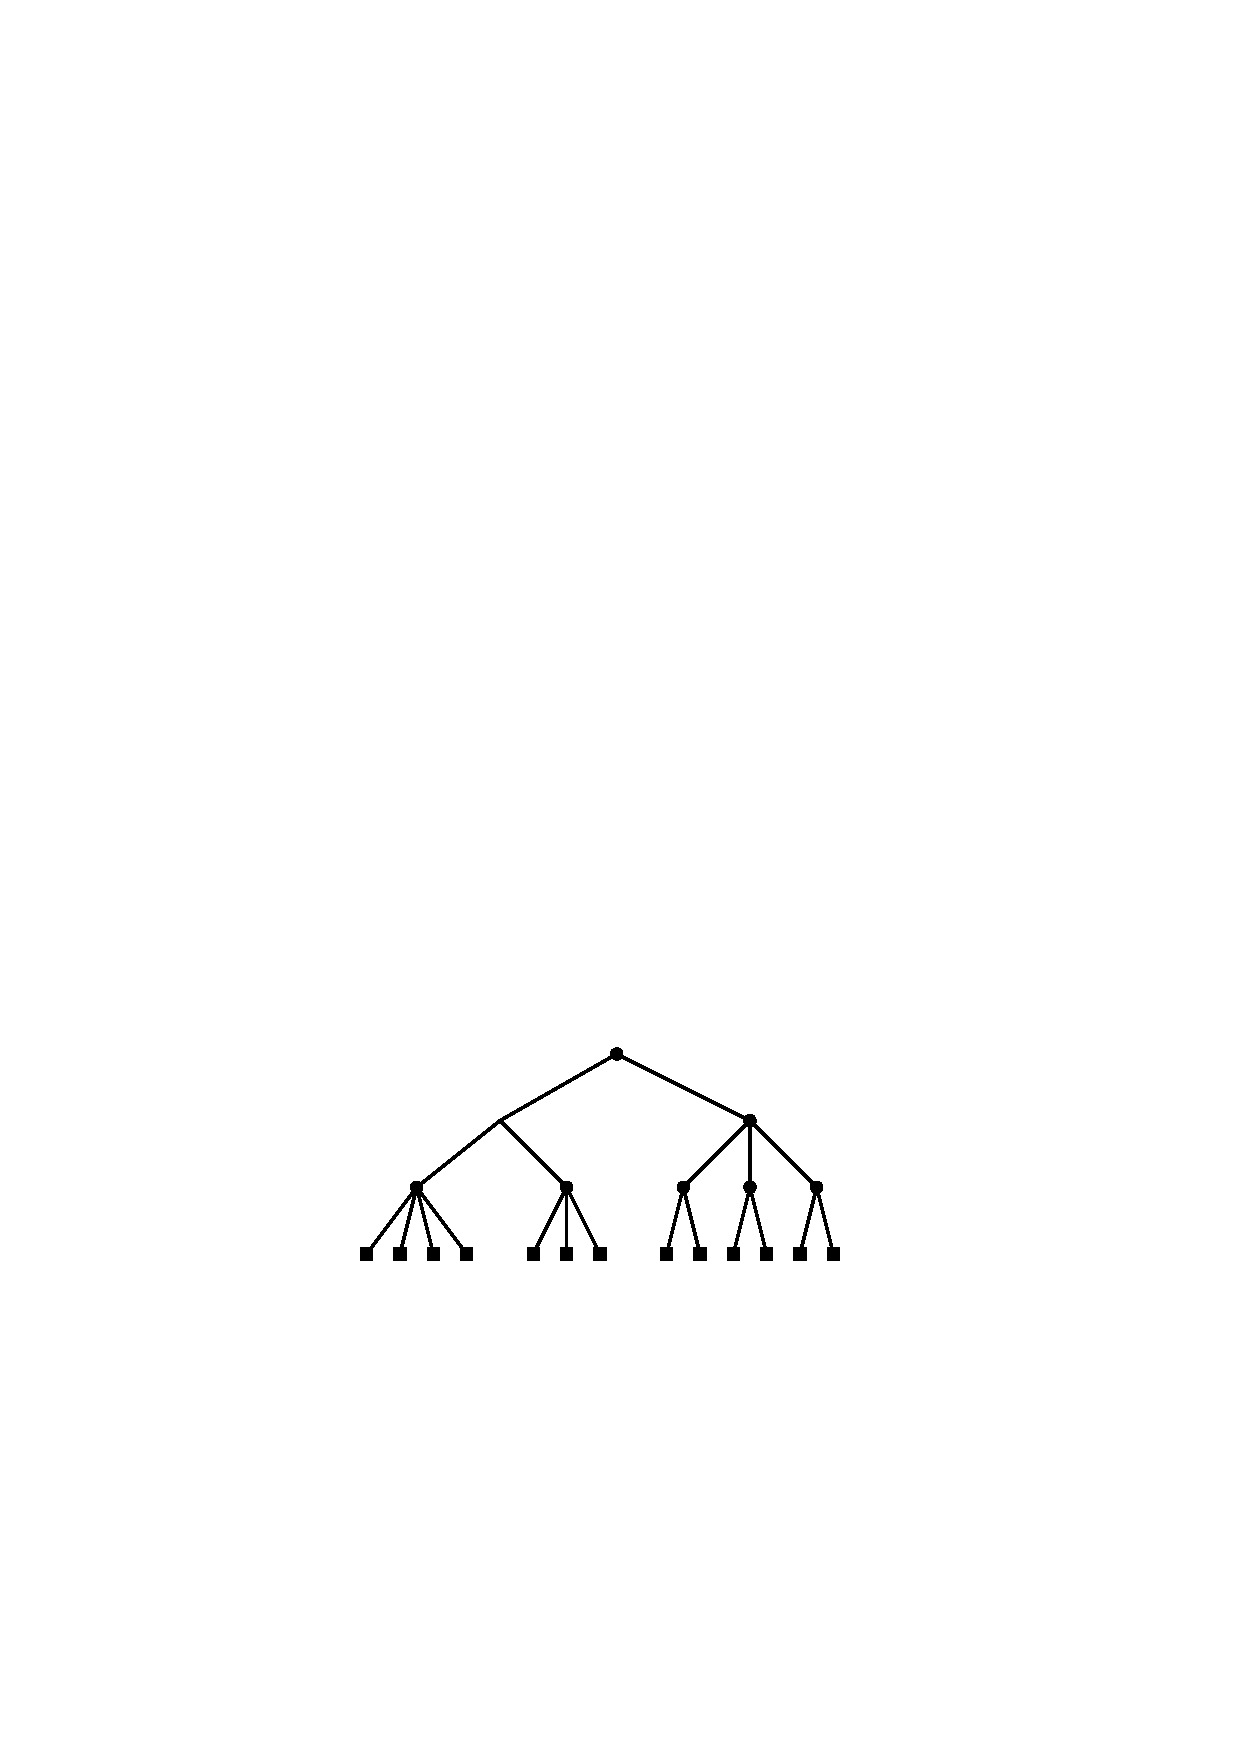
\includegraphics[scale=0.90909]{figs/24rb-2}
  \end{center}
  \caption{A 2-4 tree of height 3.}
  \figlabel{twofour-example}
\end{figure}
The properties of 2-4 trees imply that their height is logarithmic in
the number of leaves:
\begin{lem}\lemlabel{twofour-height}
  A 2-4 tree with #n# leaves has height at most $\log #n#$.
\end{lem}

\begin{proof}
  The lower-bound of 2 on the number of children of an internal node
  implies that, if the height of a 2-4 tree is $h$, then it has at least
  $2^h$ leaves.  In other words,
  \[
     #n# \ge 2^h \enspace .
  \]
  Taking logarithms on both sides of this inequality gives $h \le \log #n#$.
\end{proof}

\subsection{Adding a Leaf}

Adding a leaf to a 2-4 tree is easy (see \figref{twofour-add}).  If we
want to add a leaf #u# as the child of some node #w# on the second-last
level, then we simply make #u# a child of #w#.  This certainly maintains
the height property, but could violate the degree property;  if #w#
had four children prior to adding #u#, then #w# now has five children.
In this case, we \emph{split}
\index{split}%
#w# into two nodes, #w# and #w#', having
two and three children, respectively.
But now #w#' has no parent,
so we recursively make #w#' a child of #w#'s parent.  Again, this may
cause #w#'s parent to have too many children in which case we split it.
This process goes on until we reach a node that has fewer than four children,
or until we split the root, #r#, into two nodes #r# and #r'#.  In the
latter case, we make a new root that has #r# and #r'# as children.
This simultaneously increases the depth of all leaves and so maintains
the height property.

\begin{figure}
  \begin{center}
   \begin{tabular}{c}
     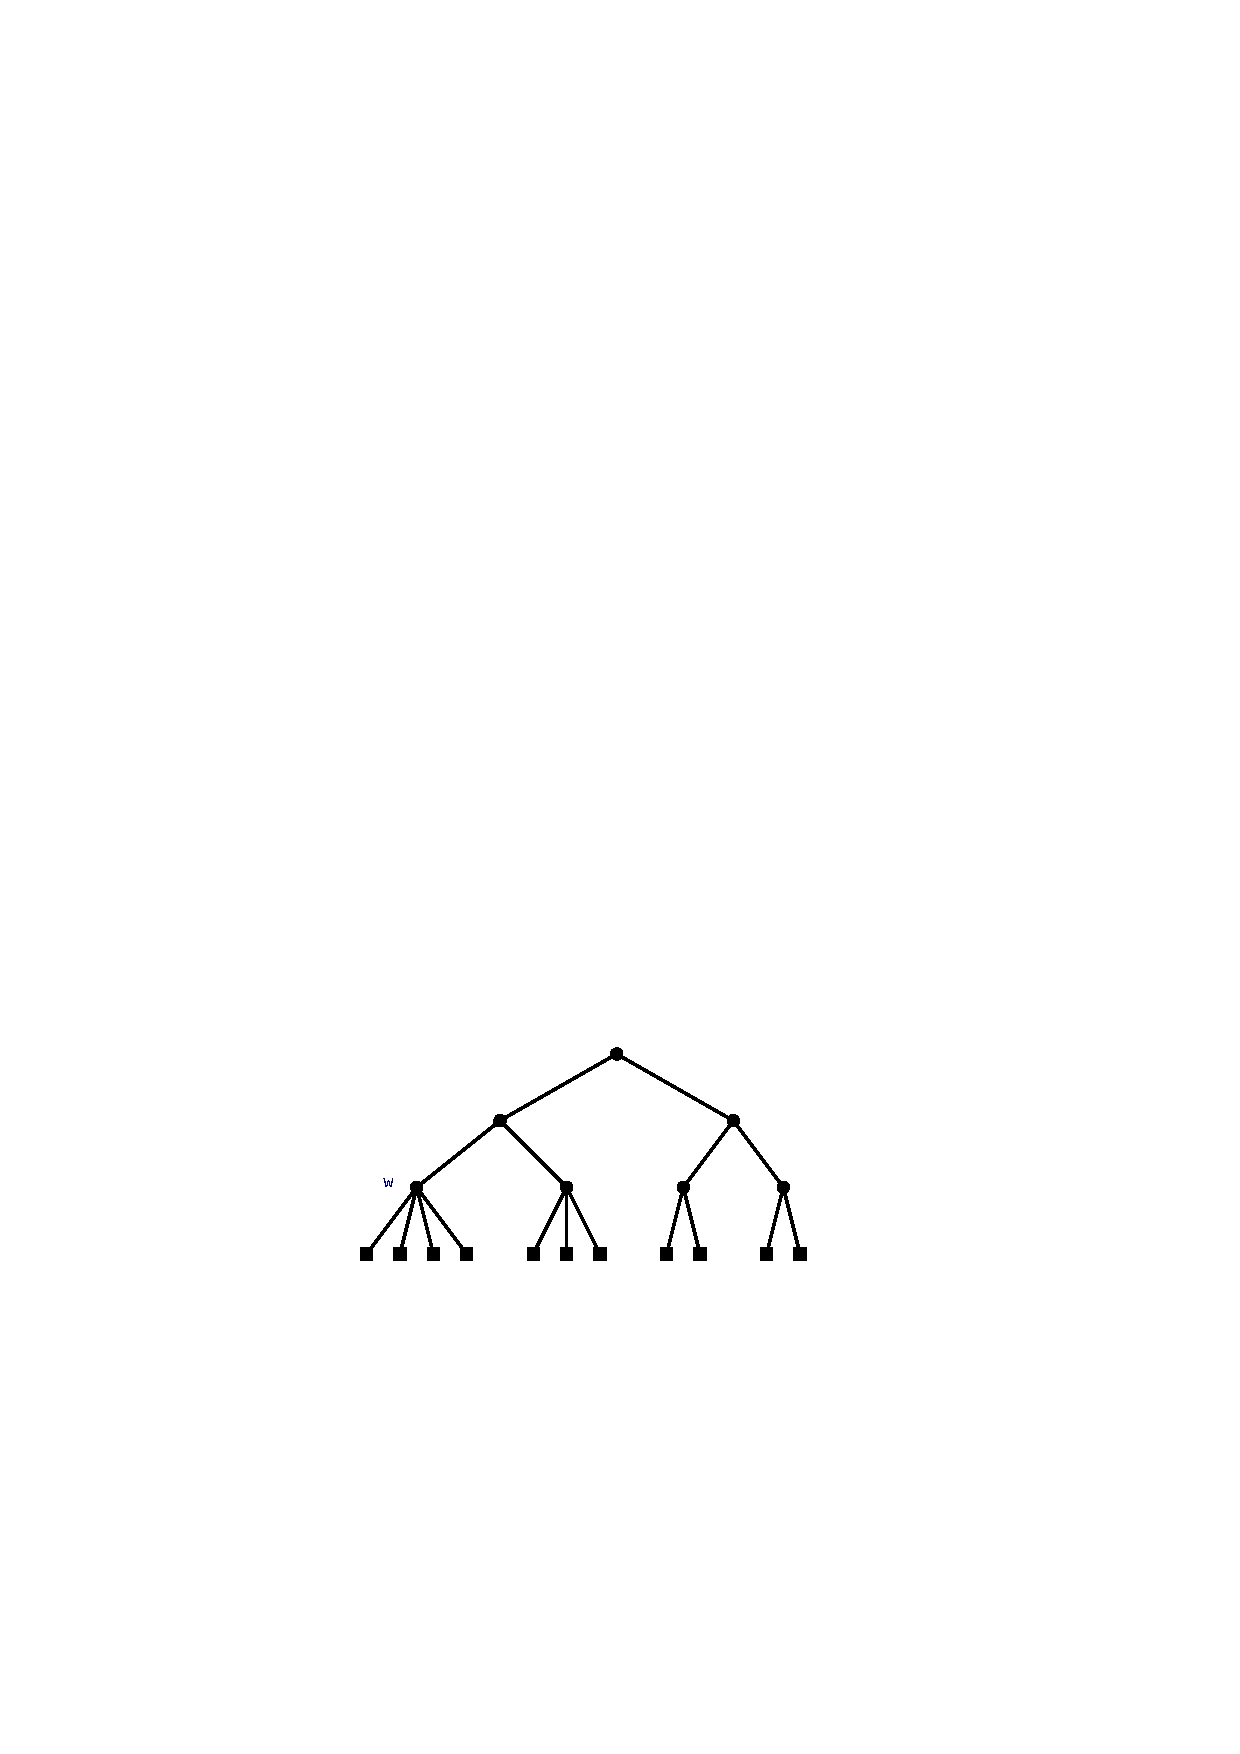
\includegraphics[scale=0.90909]{figs/24tree-add-1} \\
     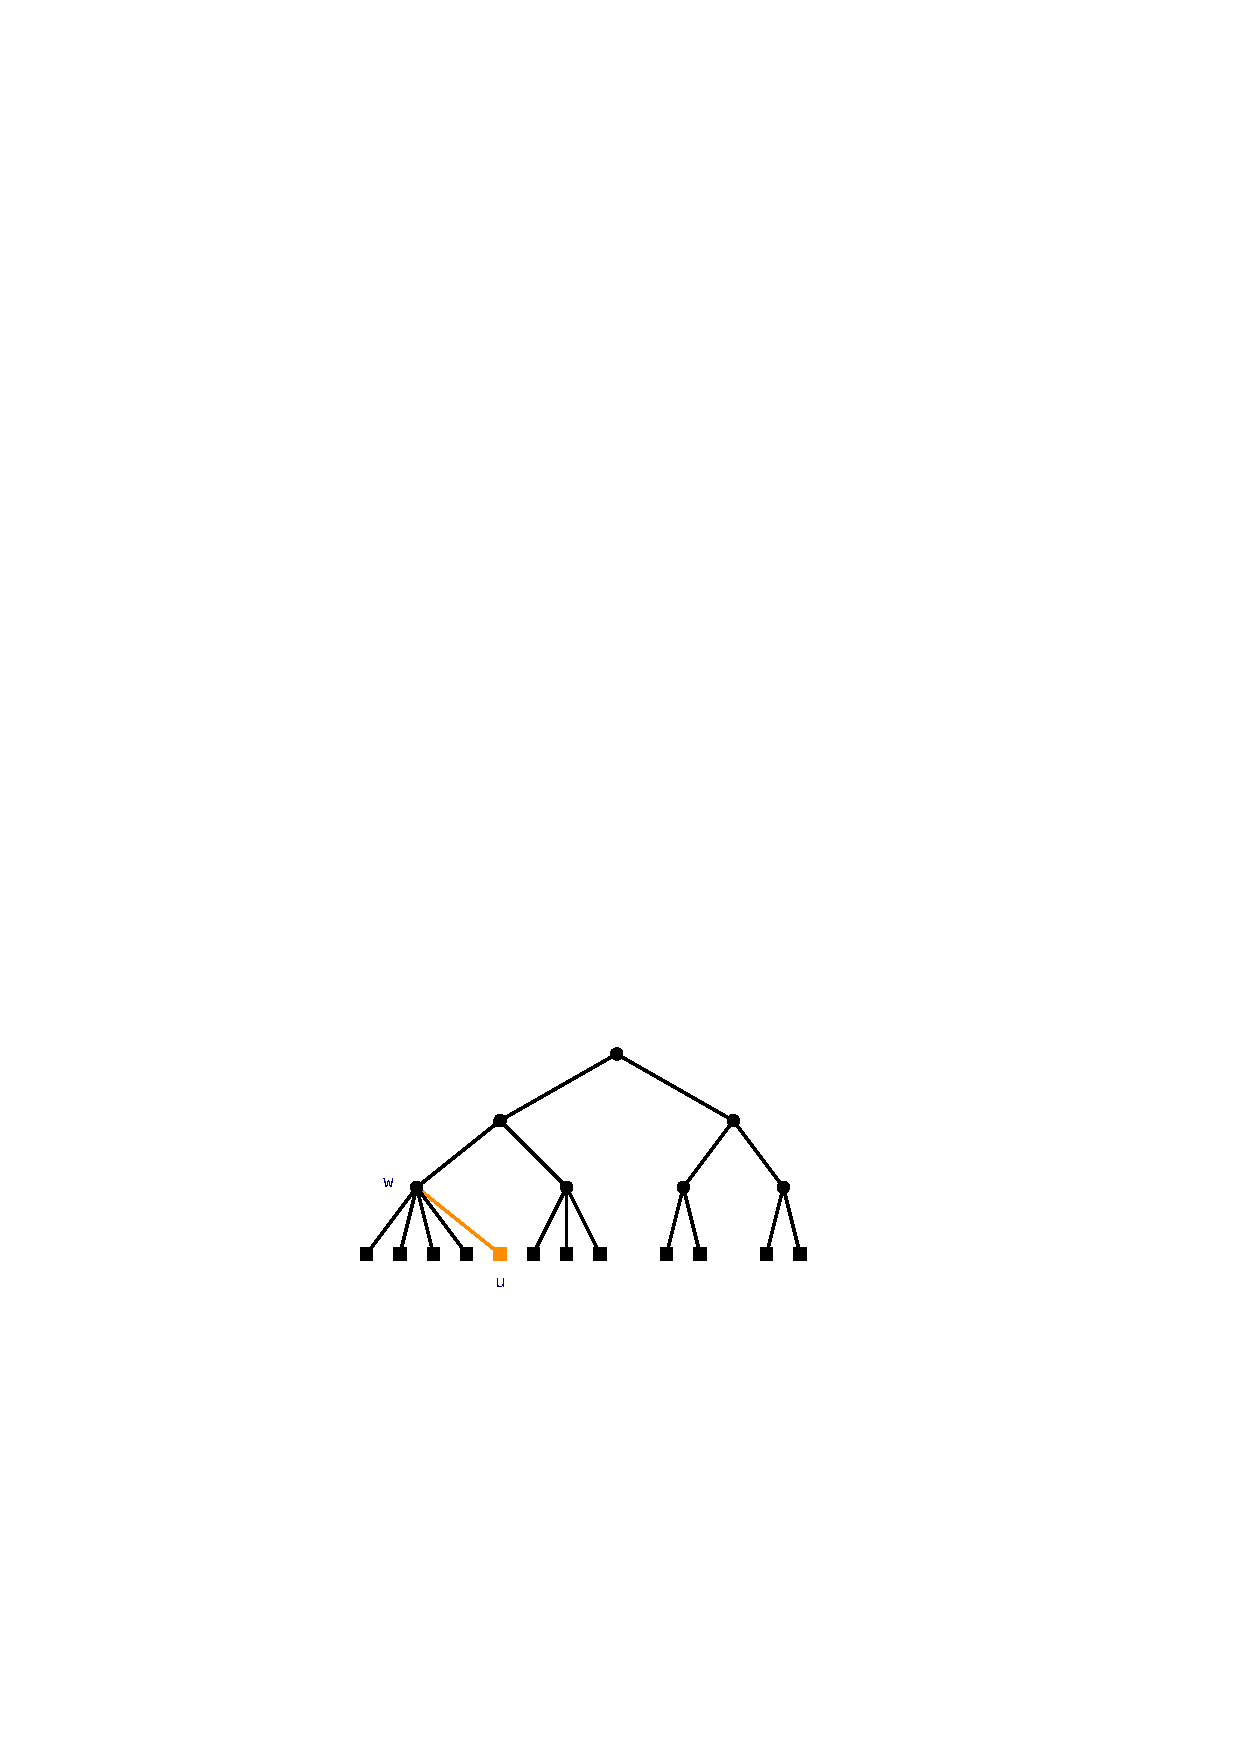
\includegraphics[scale=0.90909]{figs/24tree-add-2} \\
     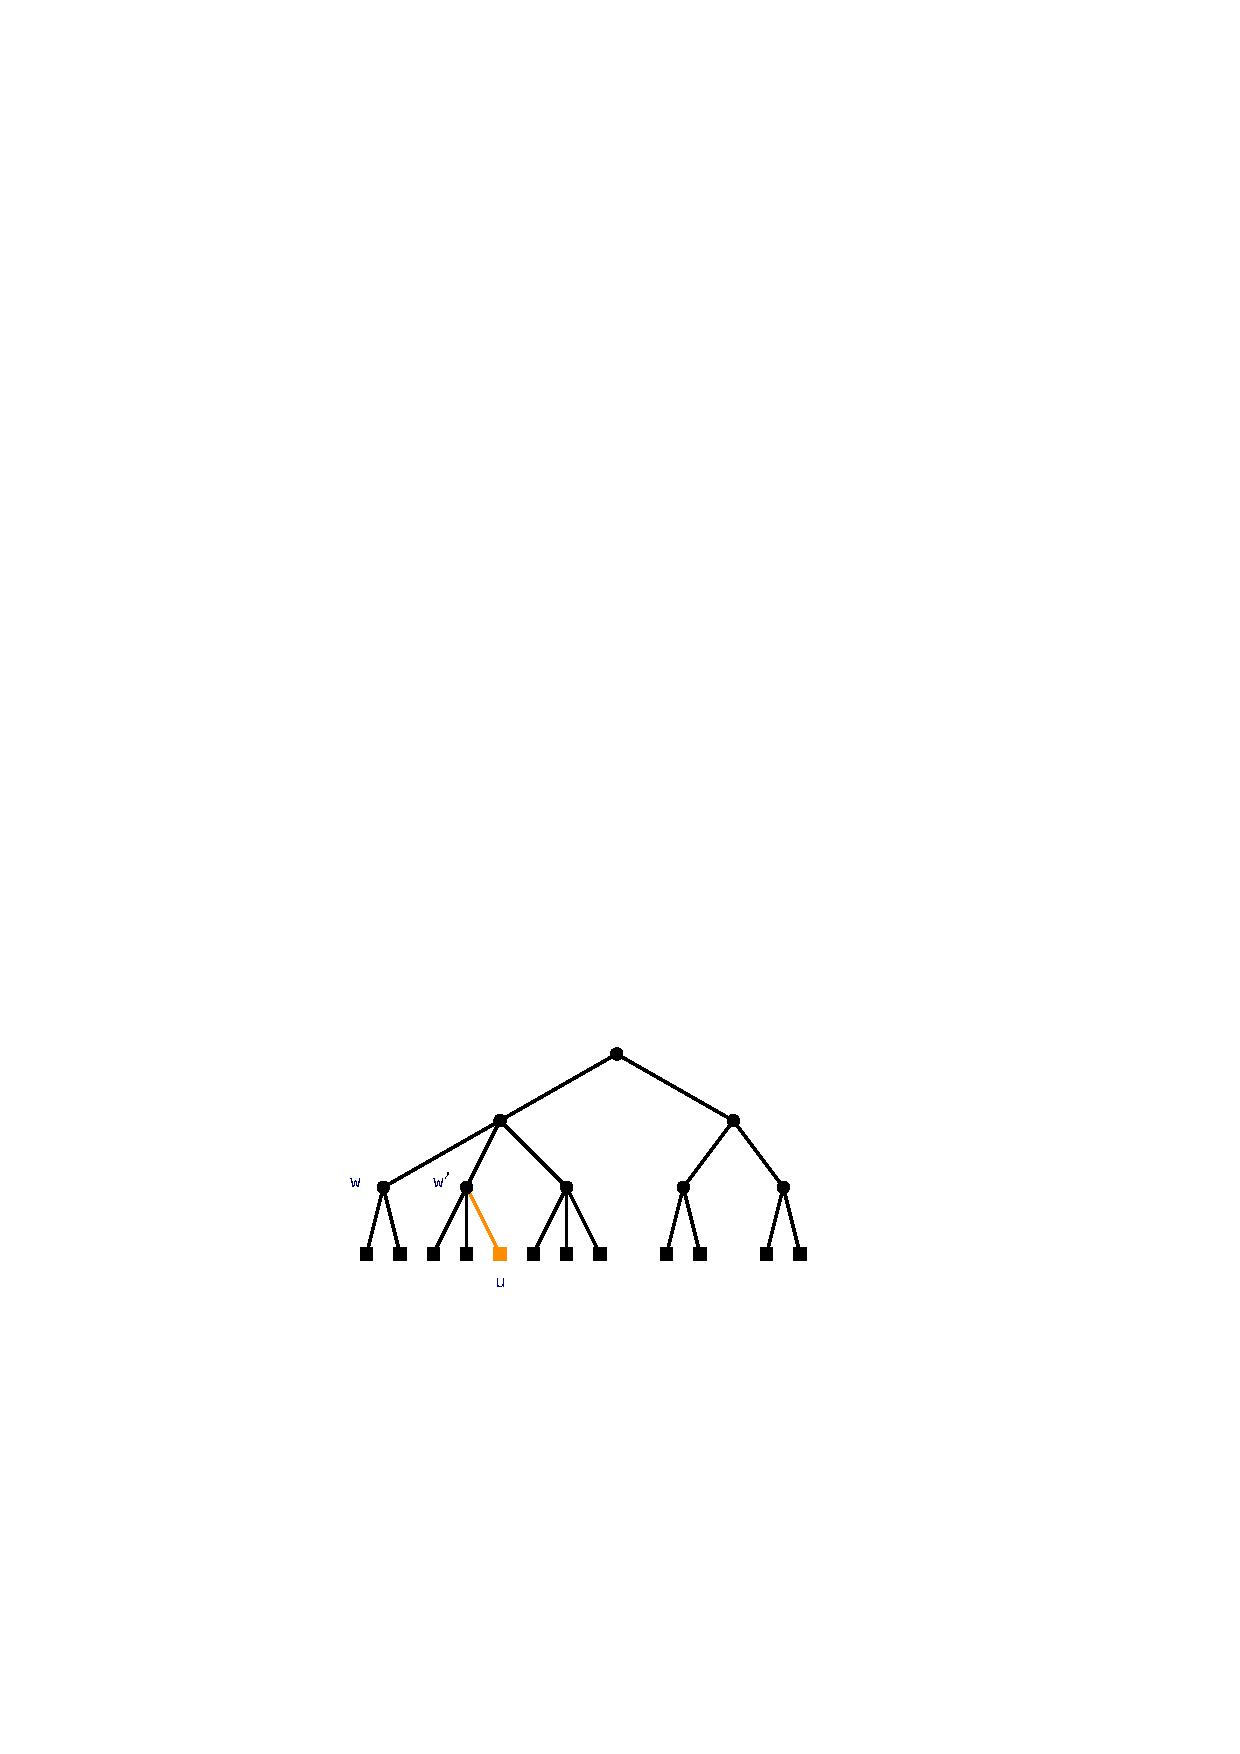
\includegraphics[scale=0.90909]{figs/24tree-add-3}
   \end{tabular}
  \end{center}
  \caption[Adding a leaf to a 2-4 Tree]{Adding a leaf to a 2-4 Tree.
  This process stops after one split because #w.parent# has a degree of less
  than 4 before the addition.}
  \figlabel{twofour-add}
\end{figure}

Since the height of the 2-4 tree is never more than $\log #n#$, the
process of adding a leaf finishes after at most $\log #n#$ steps.

\subsection{Removing a Leaf}

Removing a leaf from a 2-4 tree is a little more tricky (see
\figref{twofour-remove}).  To remove a leaf #u# from its parent #w#, we
just remove it.  If #w# had only two children prior to the removal of #u#,
then #w# is left with only one child and violates the degree property.

\begin{figure}
  \begin{center}
   \begin{tabular}{c}
     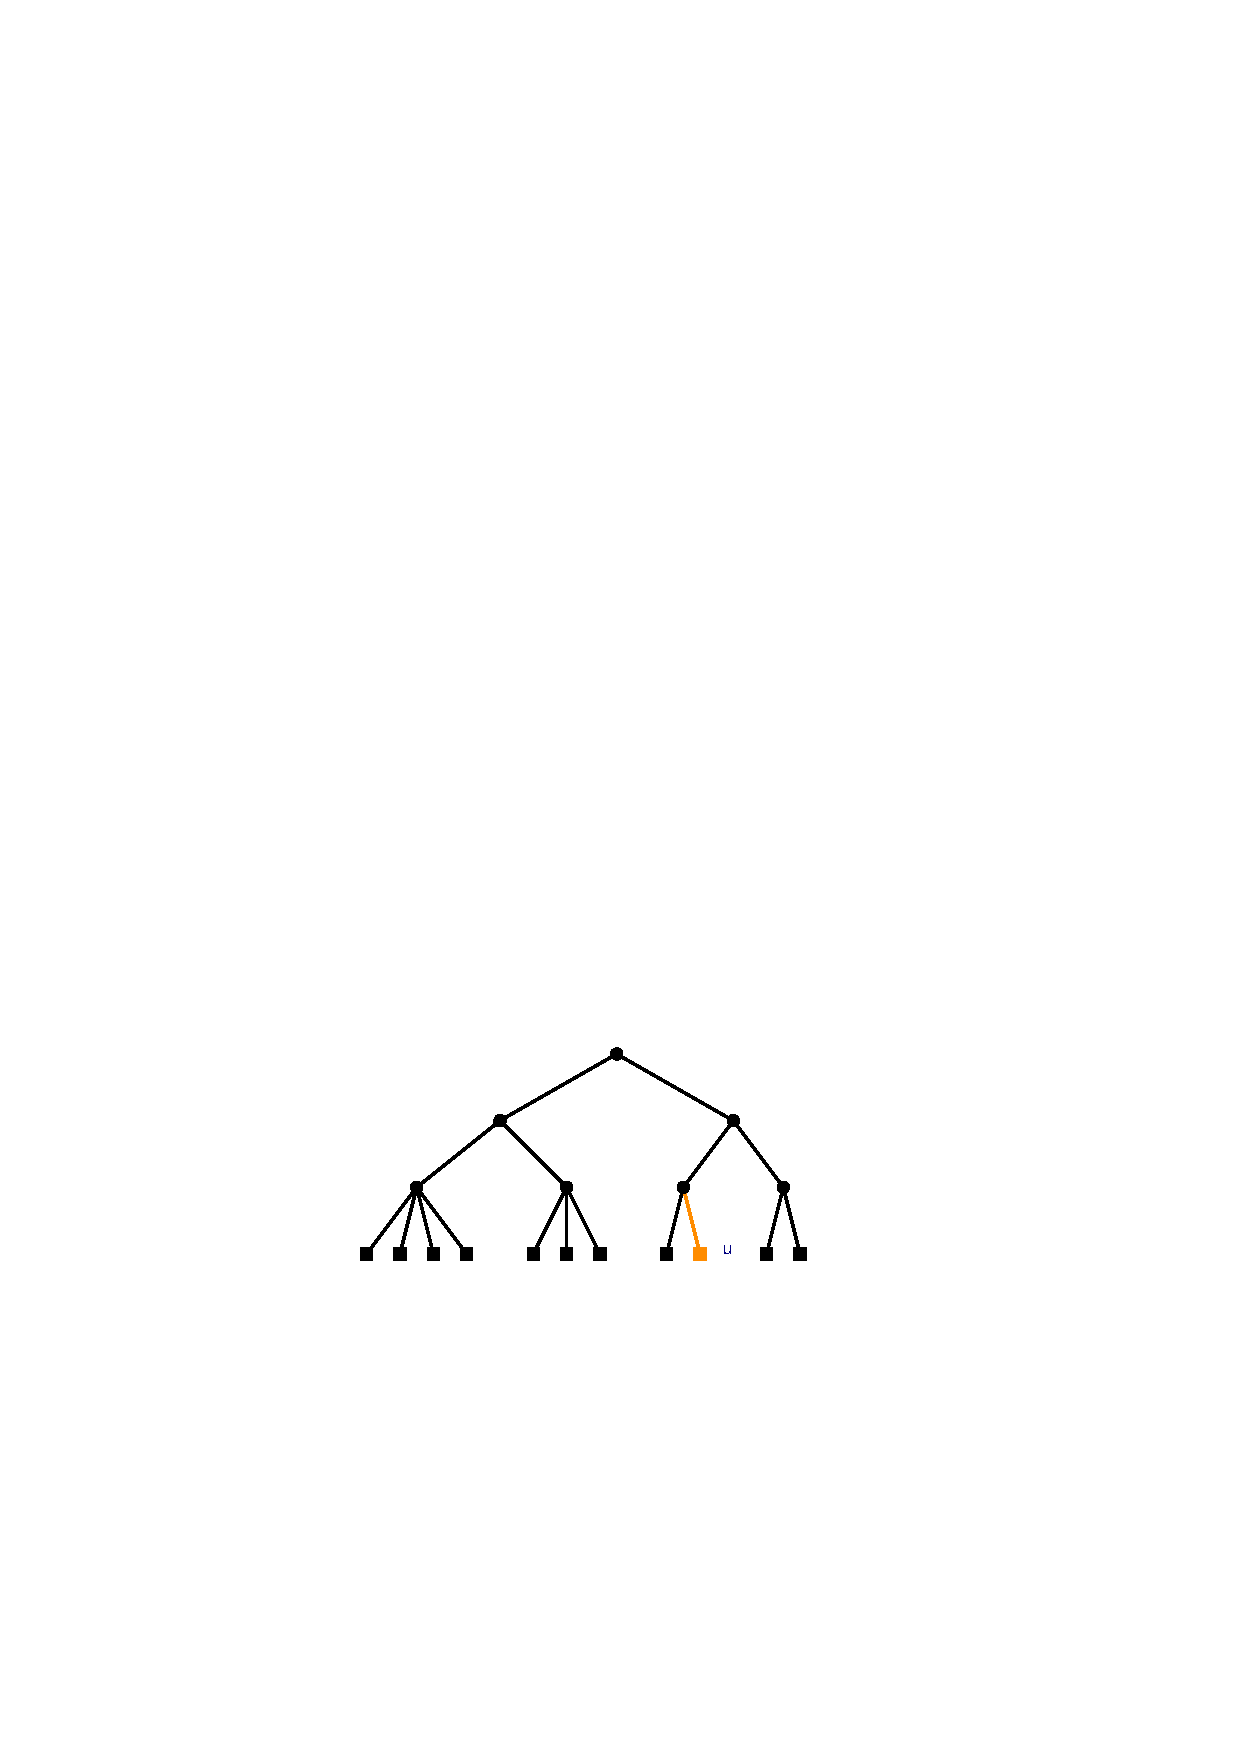
\includegraphics[height=\FifthHeightScaleIfNeeded]{figs/24tree-remove-1} \\
     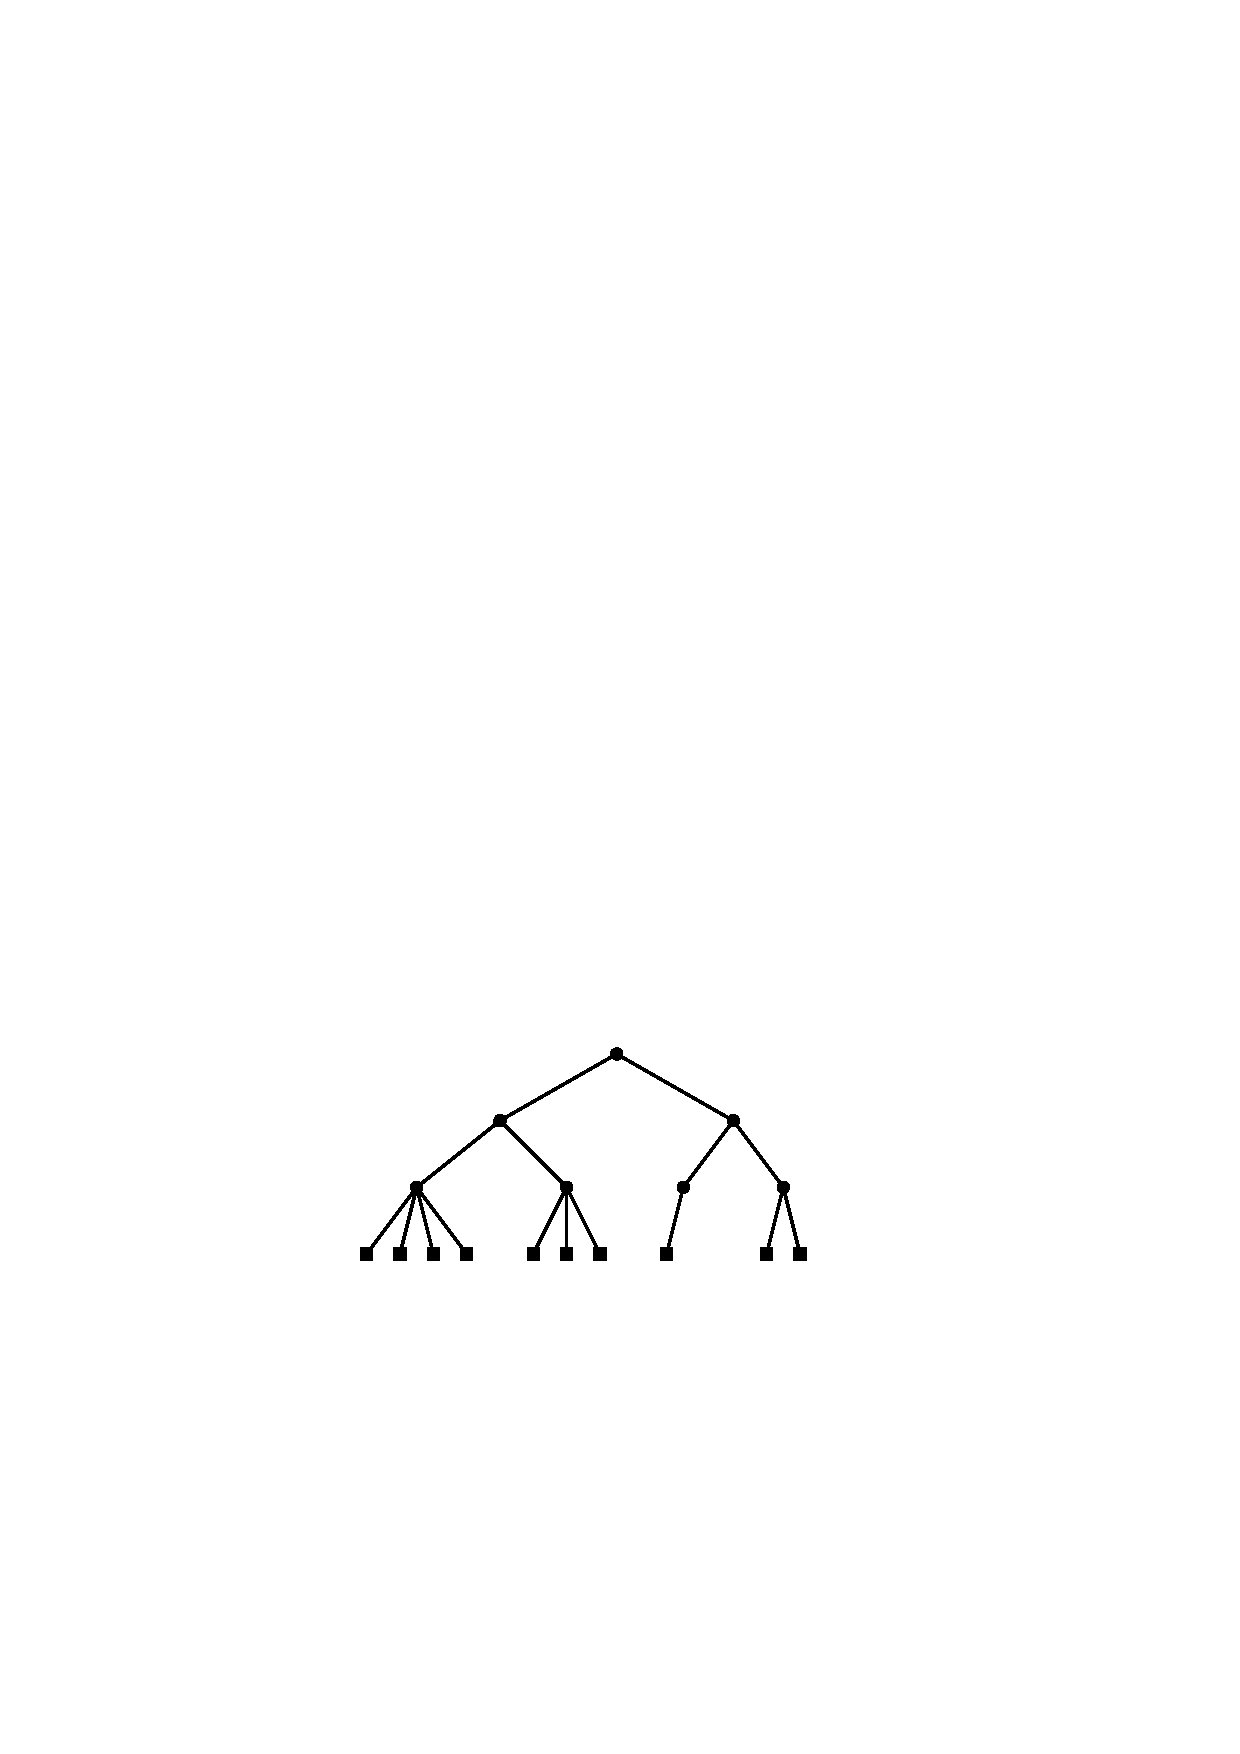
\includegraphics[height=\FifthHeightScaleIfNeeded]{figs/24tree-remove-2} \\
     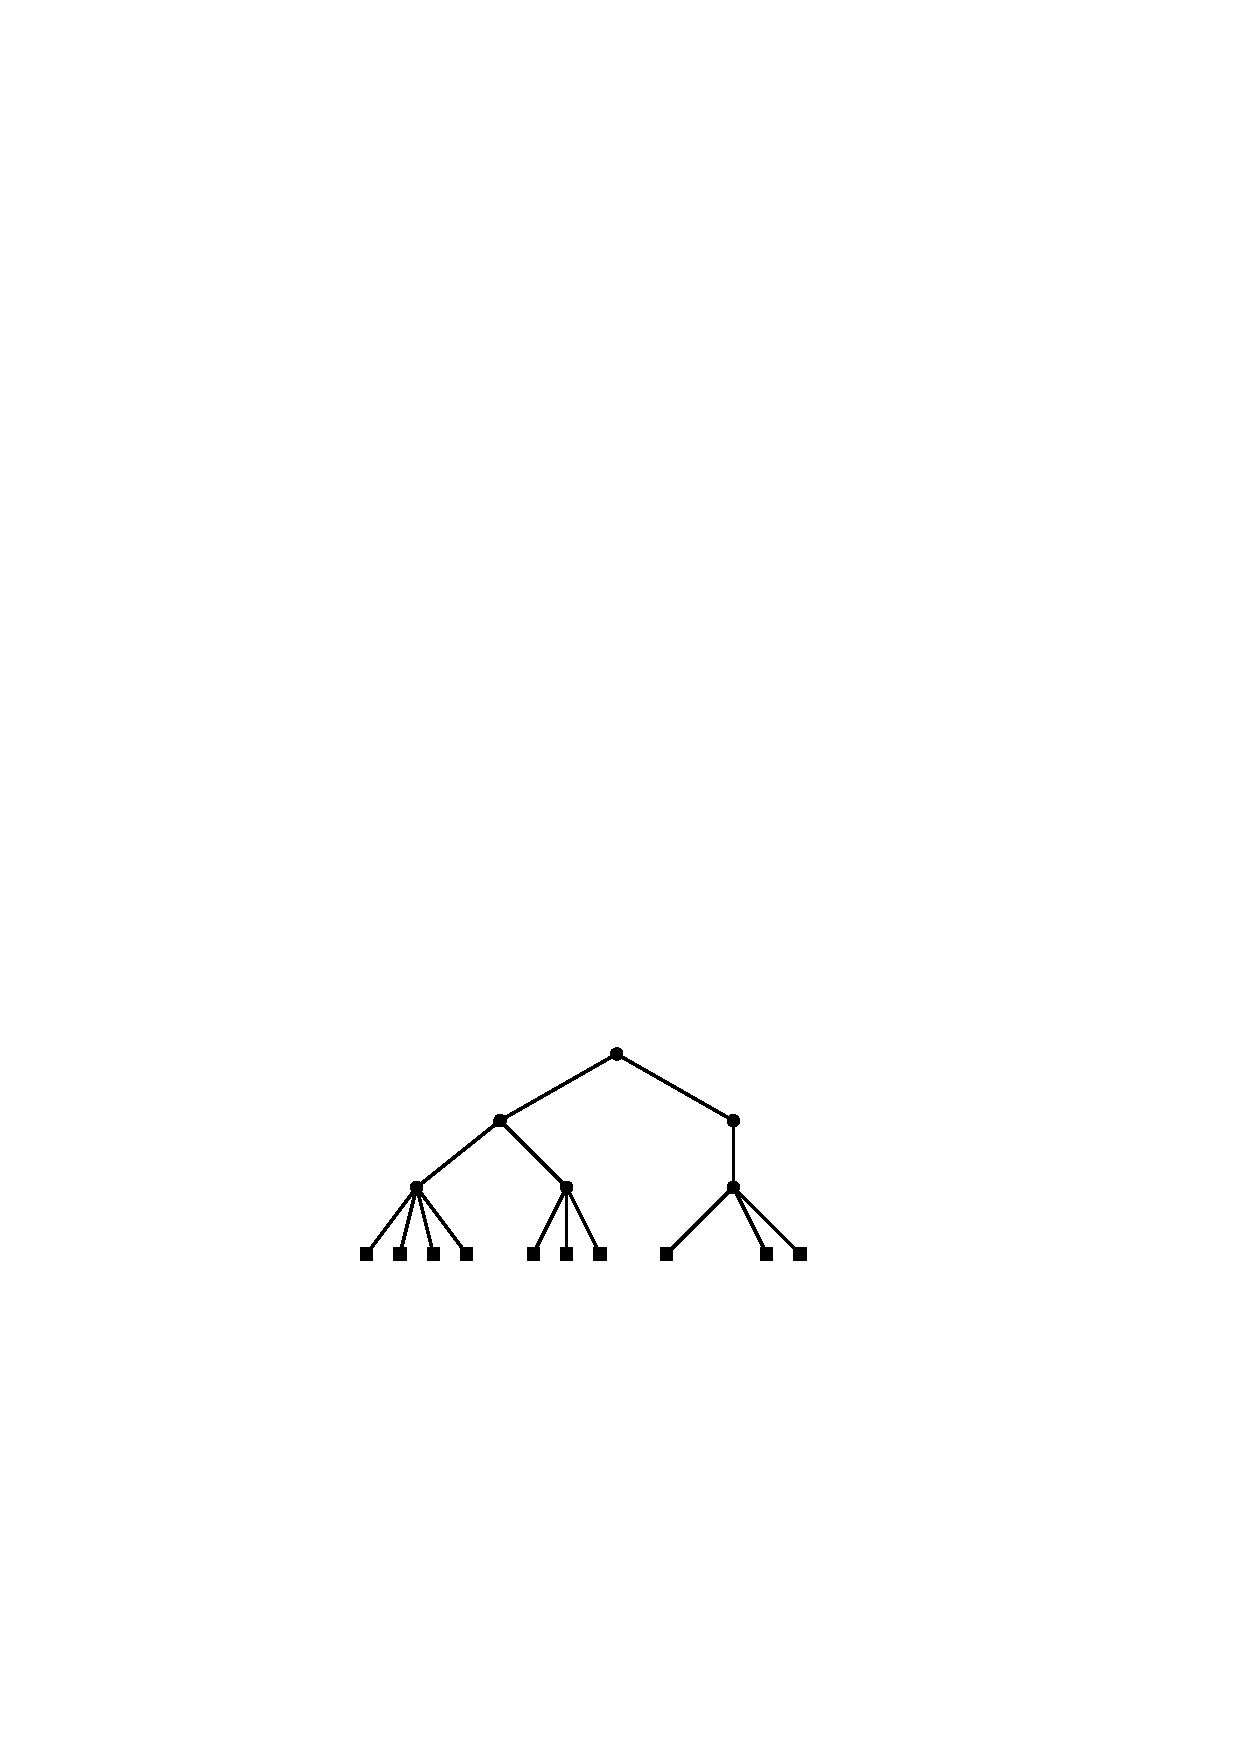
\includegraphics[height=\FifthHeightScaleIfNeeded]{figs/24tree-remove-3} \\
     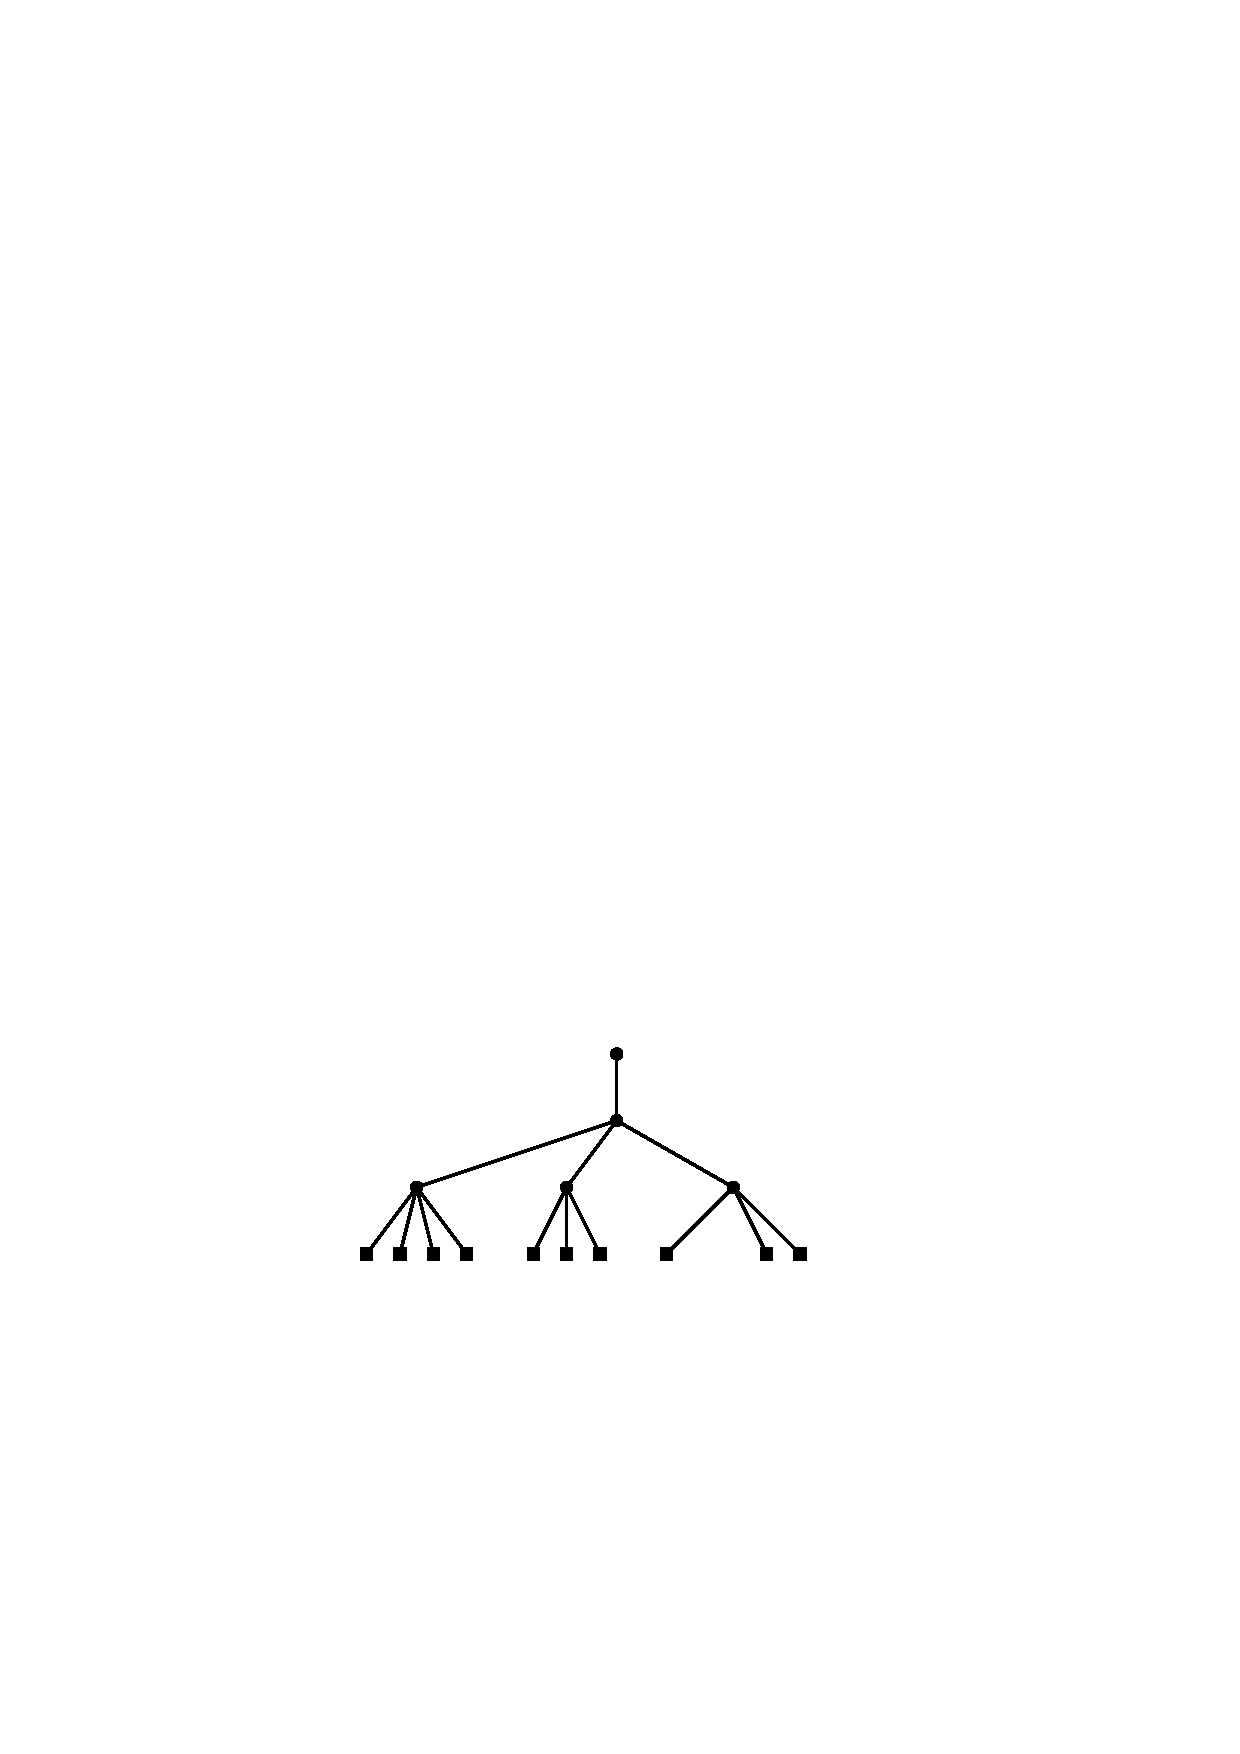
\includegraphics[height=\FifthHeightScaleIfNeeded]{figs/24tree-remove-4} \\
     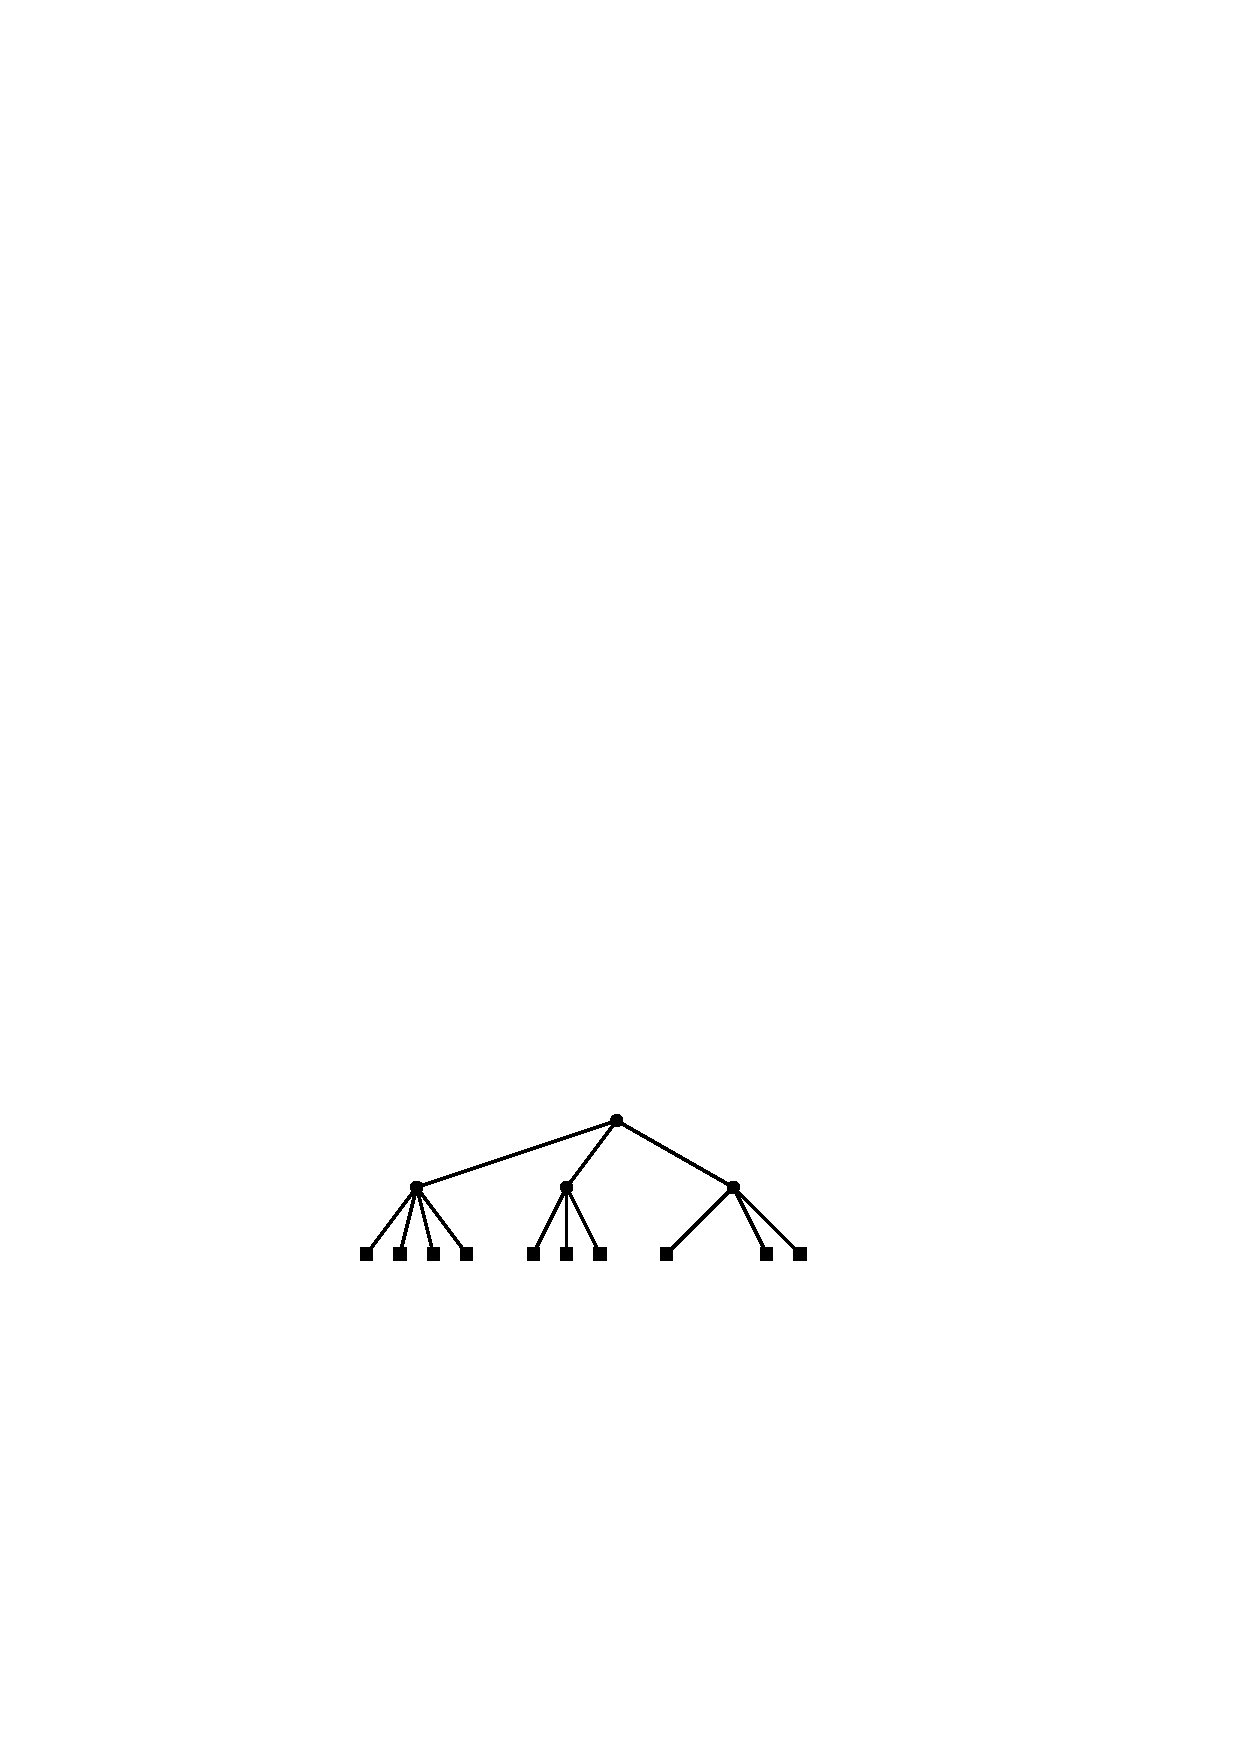
\includegraphics[height=\FifthHeightScaleIfNeeded]{figs/24tree-remove-5} \\
   \end{tabular}
  \end{center}
  \caption[Removing a leaf from a 2-4 Tree]{Removing a leaf from a
    2-4 Tree.  This process goes all the way to the root because each of
    #u#'s ancestors and their siblings have only two children.}
  \figlabel{twofour-remove}
\end{figure}

To correct this, we look at #w#'s sibling, #w'#.  The node #w'# is
sure to exist since #w#'s parent had at least two children.  If #w'#
has three or four children, then we take one of these children from #w'#
and give it to #w#. Now #w# has two children and #w'# has two or three
children and we are done.

On the other hand, if #w'# has only two children, then we \emph{merge}
\index{merge}%
#w# and #w'# into a single node, #w#, that has three children.  Next we
recursively remove #w'# from the parent of #w'#.  This process ends
when we reach a node, #u#, where #u# or its sibling has more than two
children, or when we reach the root.  In the latter case, if the root
is left with only one child, then we delete the root and make its child
the new root.  Again, this simultaneously decreases the height of every
leaf and therefore maintains the height property.

Again, since the height of the tree is never more than $\log #n#$,
the process of removing a leaf finishes after at most $\log #n#$ steps.

\section{#RedBlackTree#: A Simulated 2-4 Tree}
\seclabel{redblacktree}

A red-black tree is a binary search tree in which each node, #u#,
has a \emph{colour}
\index{colour}%
which is either \emph{red} or \emph{black}.  Red is
represented by the value $0$ and black by the value $1$.
\index{red node}%
\index{black node}%
\javaimport{ods/RedBlackTree.red.black.Node<T>}
\cppimport{ods/RedBlackTree.RedBlackNode.red.black}

Before and after any operation on a red-black tree, the following two
properties are satisfied. Each property is defined both in terms of the
colours red and black, and in terms of the numeric values 0 and 1.
\begin{prp}[black-height]
  \index{black-height property}%
  There are the same number of black nodes on every root to leaf
  path. (The sum of the colours on any root to leaf path is the same.)
\end{prp}

\begin{prp}[no-red-edge]
  \index{no-red-edge property}%
  No two red nodes are adjacent.  (For any node #u#, except the root,
  $#u.colour# + #u.parent.colour# \ge 1$.)
\end{prp}
Notice that we can always colour the root, #r#, of a red-black tree black
without violating either of these two properties, so we will assume
that the root is black, and the algorithms for updating a red-black
tree will maintain this.  Another trick that simplifies red-black trees
is to treat the external nodes (represented by #nil#) as black nodes.
This way, every real node, #u#, of a red-black tree has exactly two
children, each with a well-defined colour.  An example of a red-black
tree is shown in \figref{redblack-example}.

\begin{figure}
  \begin{center}
    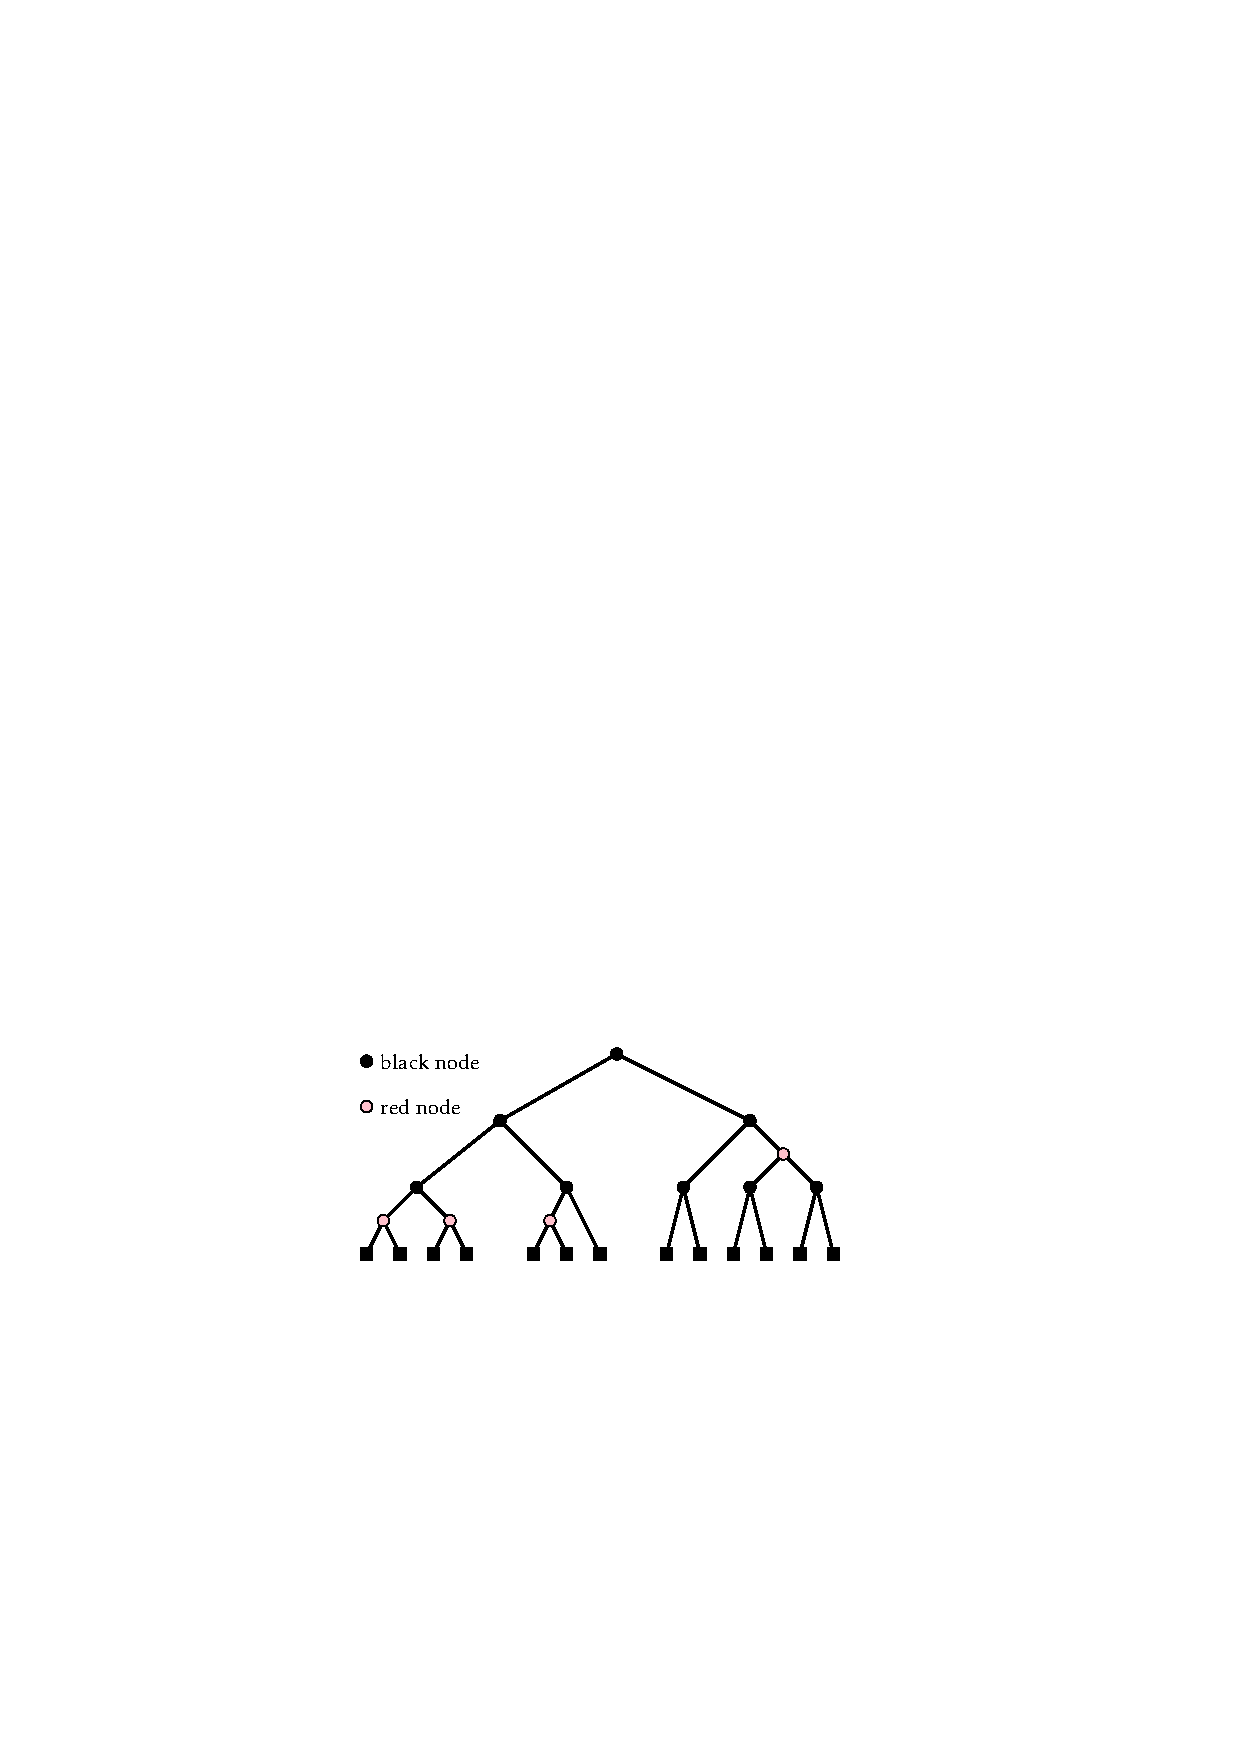
\includegraphics[scale=0.90909]{figs/24rb-1}
  \end{center}
  \caption[A red-black tree]{An example of a red-black tree with black-height 3.  External (#nil#) nodes are drawn as squares.} 
  \figlabel{redblack-example}
\end{figure}


\subsection{Red-Black Trees and 2-4 Trees}

At first it might seem surprising that a red-black tree can be efficiently
updated to maintain the black-height and no-red-edge properties, and
it seems unusual to even consider these as useful properties.  However,
red-black trees were designed to be an efficient simulation of 2-4 trees
as binary trees.

Refer to \figref{twofour-redblack}.
Consider any red-black tree, $T$, having #n# nodes and perform the
following transformation: Remove each red node #u# and connect #u#'s two
children directly to the (black) parent of #u#.  After this transformation
we are left with a tree $T'$ having only black nodes.
\begin{figure}
  \begin{center}
    \begin{tabular}{cc}
      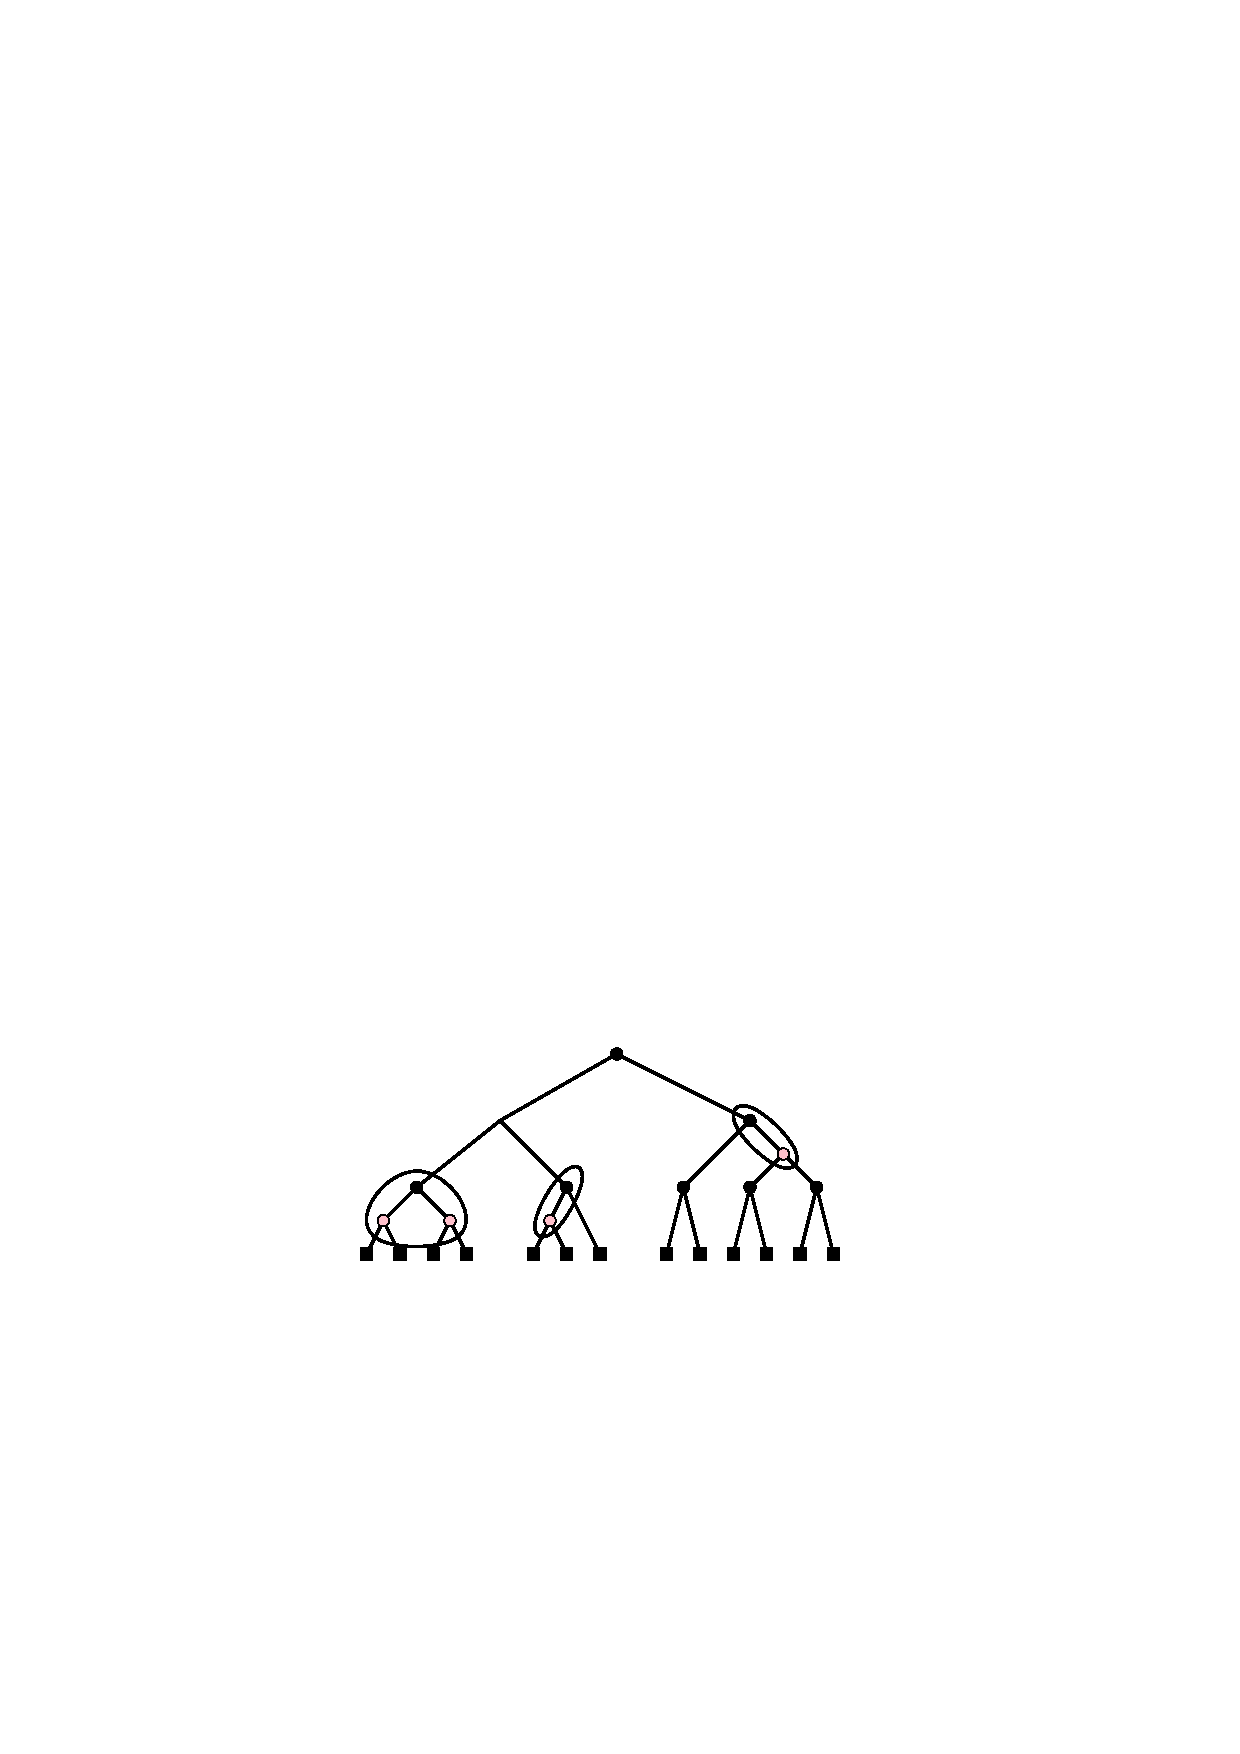
\includegraphics[scale=0.90909]{figs/24rb-3} \\
      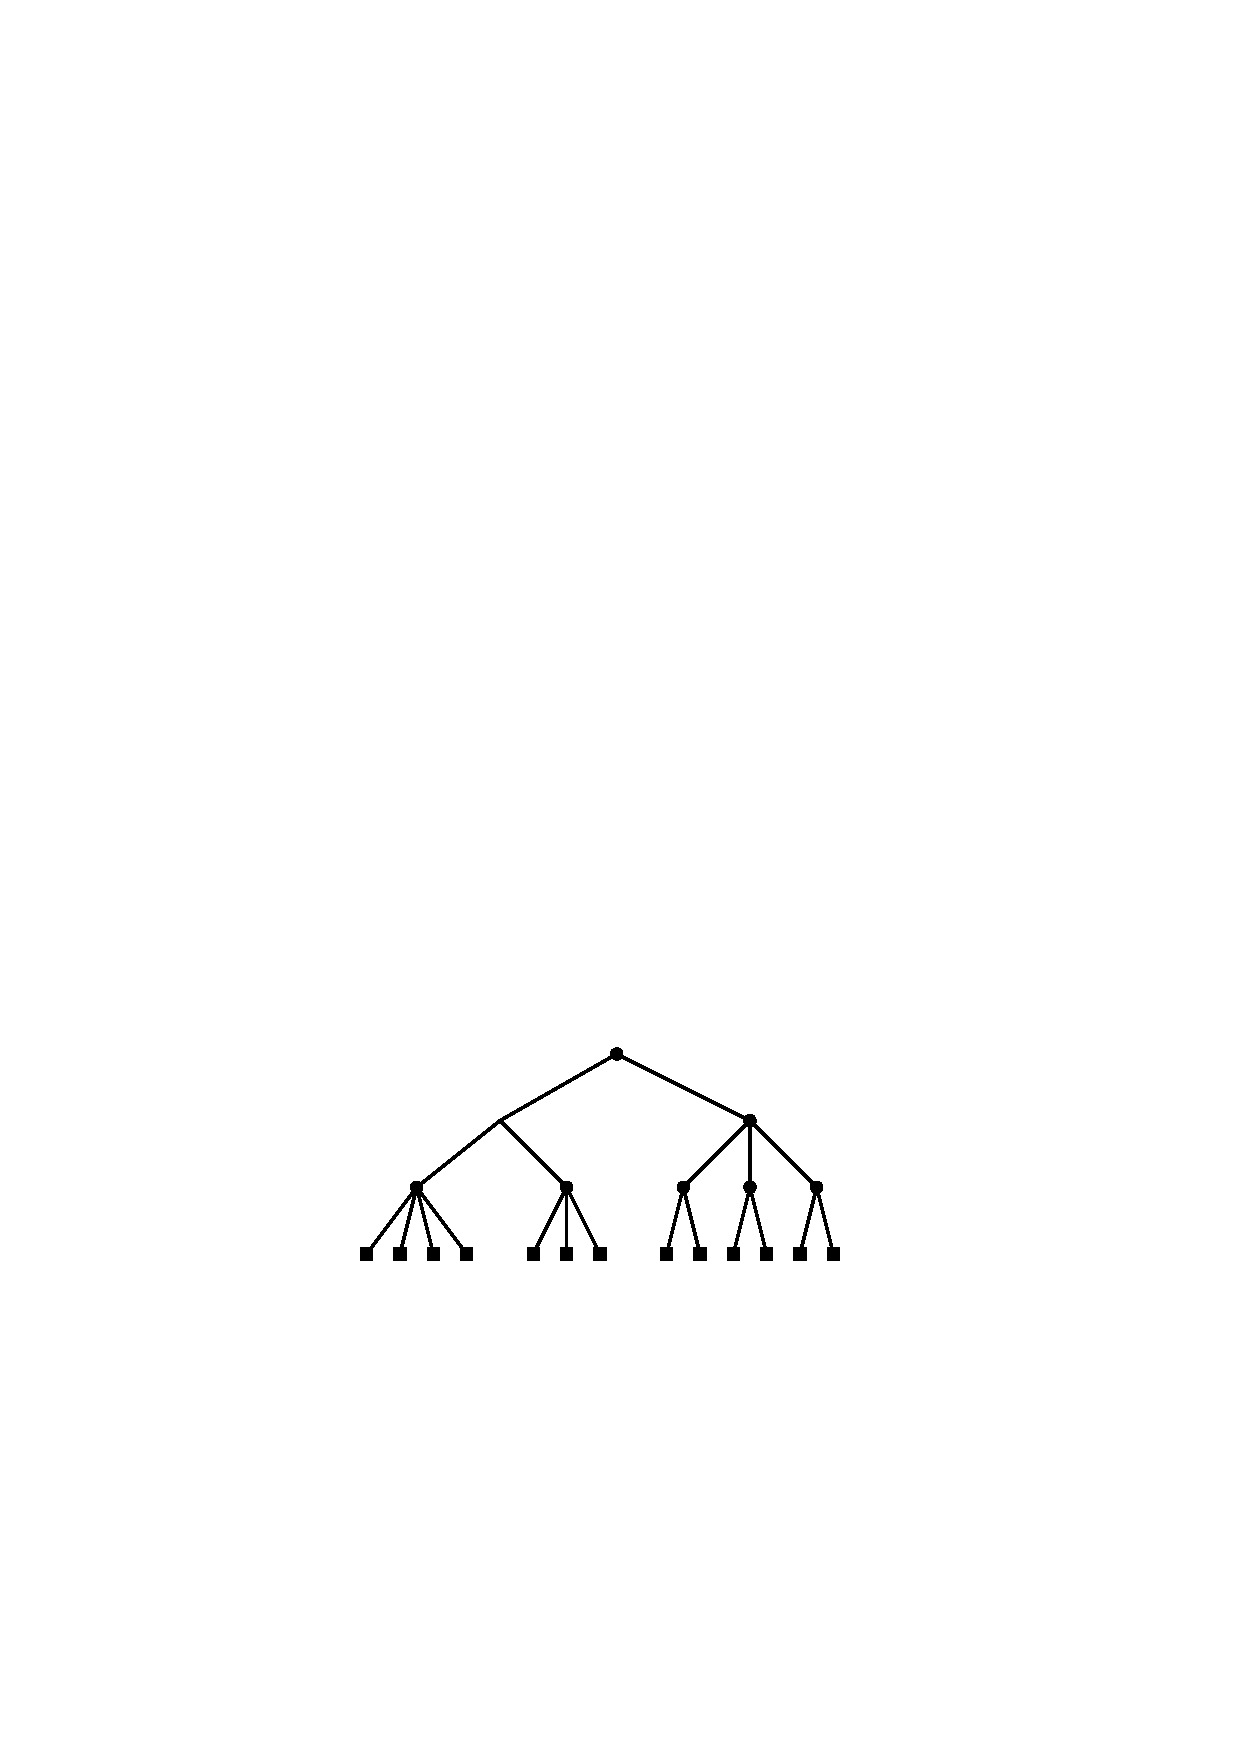
\includegraphics[scale=0.90909]{figs/24rb-2}
    \end{tabular}
  \end{center}
  \caption{Every red-black tree has a corresponding 2-4 tree.}
  \figlabel{twofour-redblack}
\end{figure}

Every internal node in $T'$ has two, three, or four children: A black
node that started out with two black children will still have two
black children after this transformation.  A black node that started
out with one red and one black child will have three children after this
transformation.  A black node that started out with two red children will
have four children after this transformation.  Furthermore, the black-height
property now guarantees that every root-to-leaf path in $T'$ has the
same length.  In other words, $T'$ is a 2-4 tree!

The 2-4 tree $T'$ has $#n#+1$ leaves that correspond to the $#n#+1$
external nodes of the red-black tree.  Therefore, this tree has height
at most $\log (#n#+1)$. Now, every root to leaf path in the 2-4 tree corresponds
to a path from the root of the red-black tree $T$ to an external node.
The first and last node in this path are black and at most one out of
every two internal nodes is red, so this path has at most $\log(#n#+1)$
black nodes and at most $\log(#n#+1)-1$ red nodes.  Therefore, the longest path from the root to any \emph{internal} node in $T$ is at most
\[
   2\log(#n#+1) -2 \le 2\log #n# \enspace ,
\]
for any $#n#\ge 1$.  This proves the most important property of
red-black trees:
\begin{lem}
The height of red-black tree with #n# nodes is at most $2\log #n#$.
\end{lem}

Now that we have seen the relationship between 2-4 trees and
red-black trees, it is not hard to believe that we can efficiently
maintain a red-black tree while adding and removing elements.  

We have already seen that adding an element in a #BinarySearchTree#
can be done by adding a new leaf.  Therefore, to implement #add(x)# in a
red-black tree we need a method of simulating splitting a node with five
children in a 2-4 tree.  A 2-4 tree node with five children is represented
by a black node that has two red children, one of which also has a red
child. We can ``split'' this node by colouring it red and colouring its
two children black.  An example of this is shown in \figref{rb-split}.

\begin{figure}
  \begin{center}
   \begin{tabular}{c}
     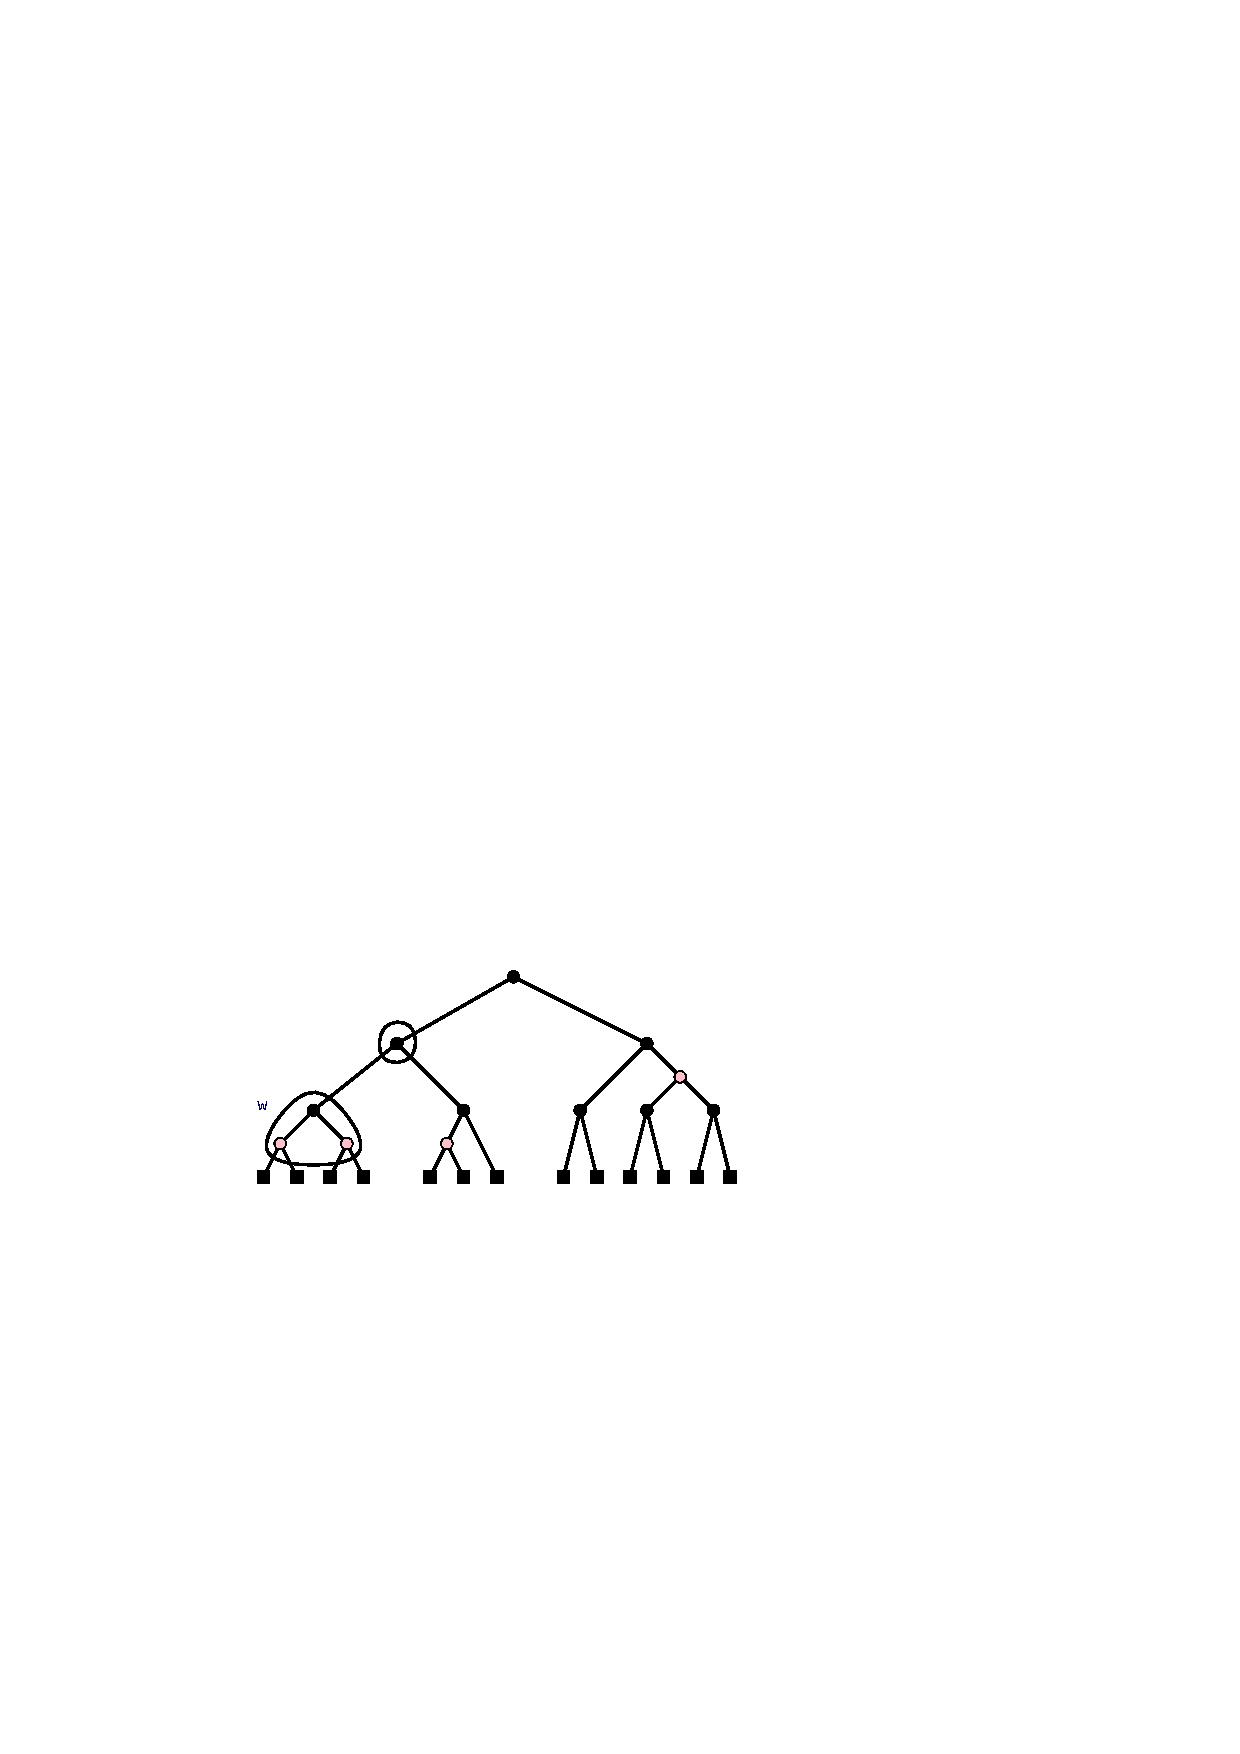
\includegraphics[scale=0.90909]{figs/rb-split-1} \\
     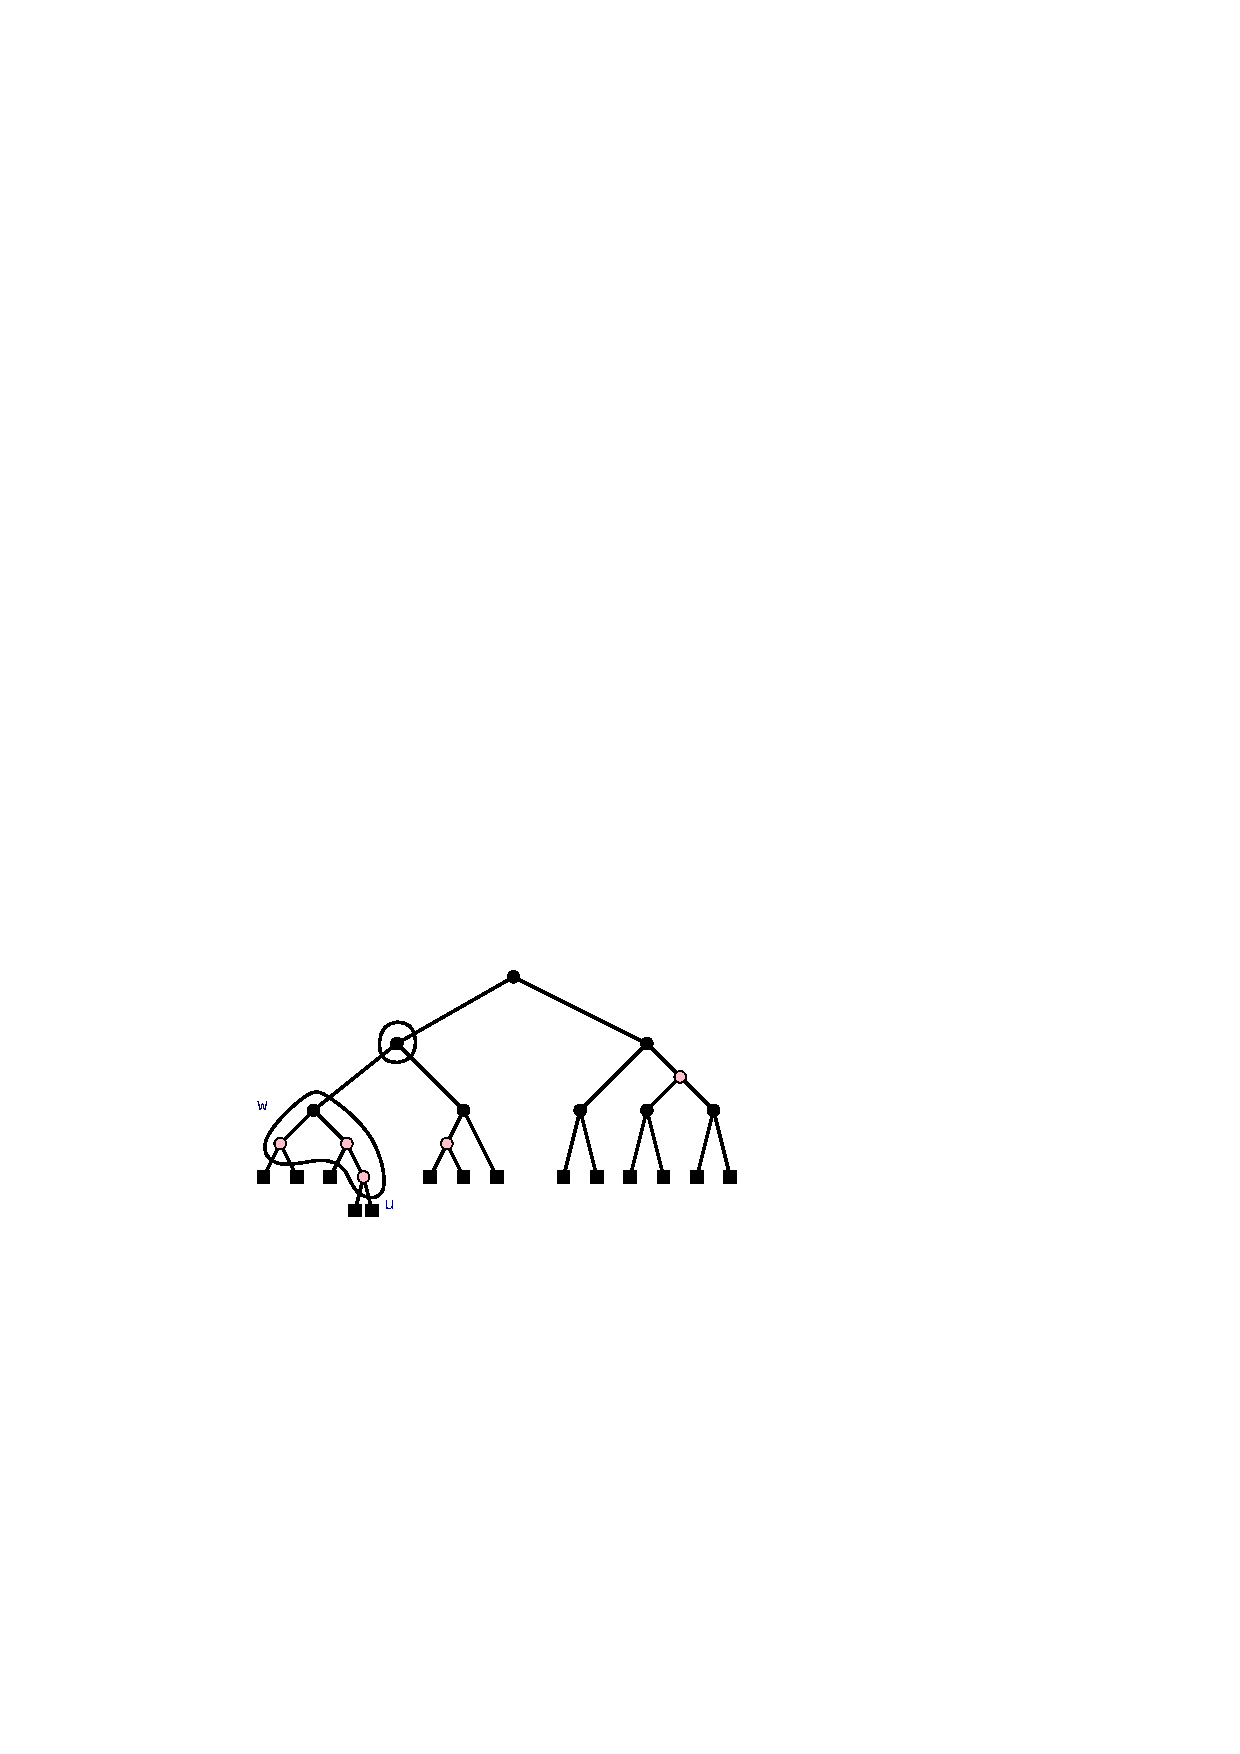
\includegraphics[scale=0.90909]{figs/rb-split-2} \\
     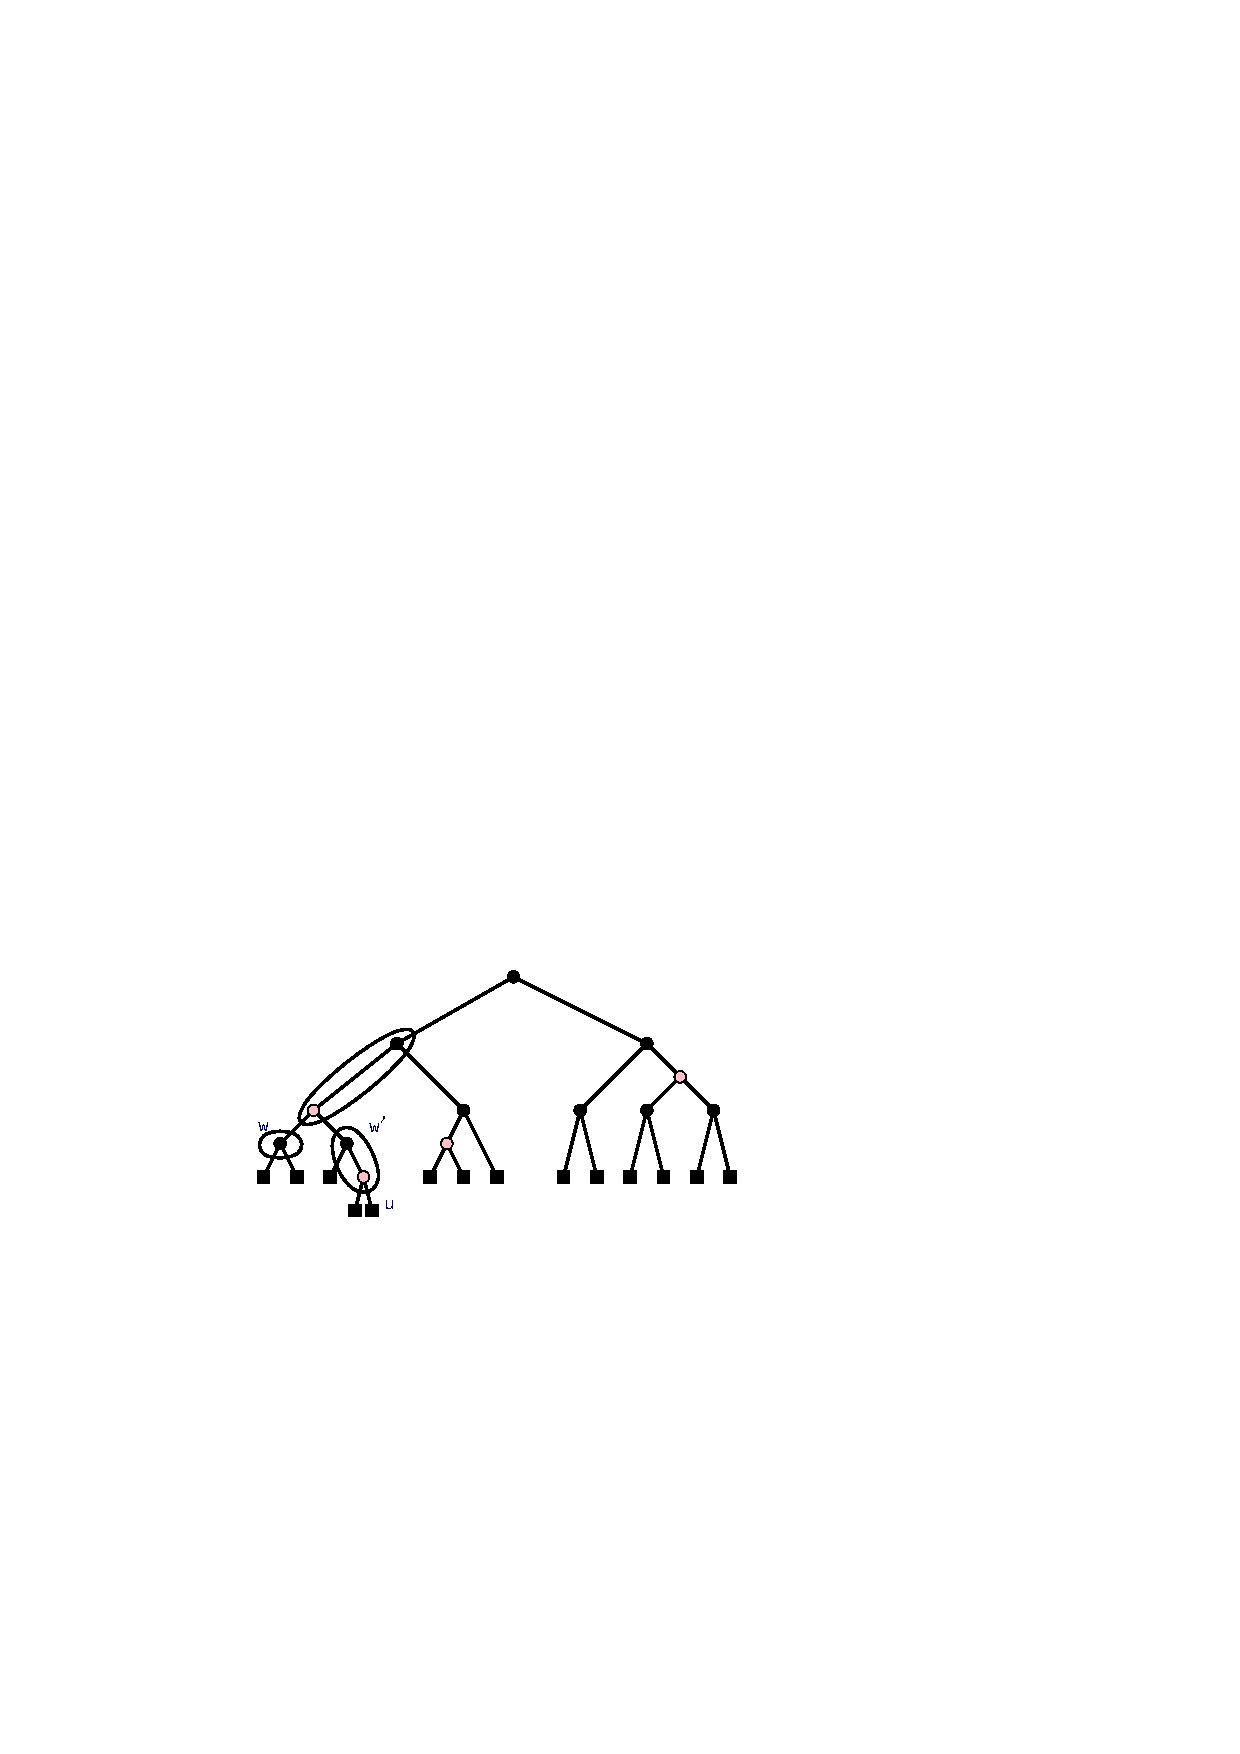
\includegraphics[scale=0.90909]{figs/rb-split-3} \\
   \end{tabular}
  \end{center}
  \caption[Simulating a 2-4 tree]{Simulating a 2-4 tree split operation
    during an addition in a red-black tree.  (This simulates the 2-4
    tree addition shown in \figref{twofour-add}.)}
  \figlabel{rb-split}
\end{figure}

Similarly, implementing #remove(x)# requires a method of merging two nodes
and borrowing a child from a sibling.  Merging two nodes is the inverse of
a split (shown in \figref{rb-split}), and involves colouring two (black)
siblings red and colouring their (red) parent black.  Borrowing from
a sibling is the most complicated of the procedures and involves both
rotations and recolouring nodes.

Of course, during all of this we must still maintain the no-red-edge
property and the black-height property.  While it is no longer surprising
that this can be done, there are a large number of cases that have to
be considered if we try to do a direct simulation of a 2-4 tree by a
red-black tree.  At some point, it just becomes simpler to disregard the
underlying 2-4 tree and work directly towards maintaining the properties
of the red-black tree.

\subsection{Left-Leaning Red-Black Trees}

\index{red-black tree}%
\index{left-leaning red-black tree}%
No single definition of red-black trees exists.  Rather, there is
a family of structures that manage to maintain the black-height
and no-red-edge properties during #add(x)# and #remove(x)#
operations. Different structures do this in different ways.
Here, we implement a data structure that we call a #RedBlackTree#.
\index{RedBlackTree@#RedBlackTree#}%
This structure implements a particular variant of red-black trees that
satisfies an additional property:
\begin{prp}[left-leaning]\prplabel{left-leaning}\prplabel{redblack-last}
  \index{left-leaning property}%
  At any node #u#, if #u.left# is black, then #u.right# is black.
\end{prp}
Note that the red-black tree shown in \figref{redblack-example}  does
not satisfy the left-leaning property;  it is violated by the parent of
the red node in the rightmost path.

The reason for maintaining the left-leaning property is that it reduces
the number of cases encountered when updating the tree during #add(x)#
and #remove(x)# operations.  In terms of 2-4 trees, it implies that every
2-4 tree has a unique representation:  A node of degree two becomes
a black node with two black children.  A node of degree three becomes
a black node whose left child is red and whose right child is black.
A node of degree four becomes a black node with two red children.

Before we describe the implementation of #add(x)# and #remove(x)# in
detail, we first present some simple subroutines used by these methods
that are illustrated in \figref{redblack-flippullpush}.  The first two
subroutines are for manipulating colours while preserving the black-height
property. The #pushBlack(u)# method takes as input a black node #u#
that has two red children and colours #u# red and its two children black.
The #pullBlack(u)# method reverses this operation:
\codeimport{ods/RedBlackTree.pushBlack(u).pullBlack(u)}

\begin{figure}
  \begin{center}
    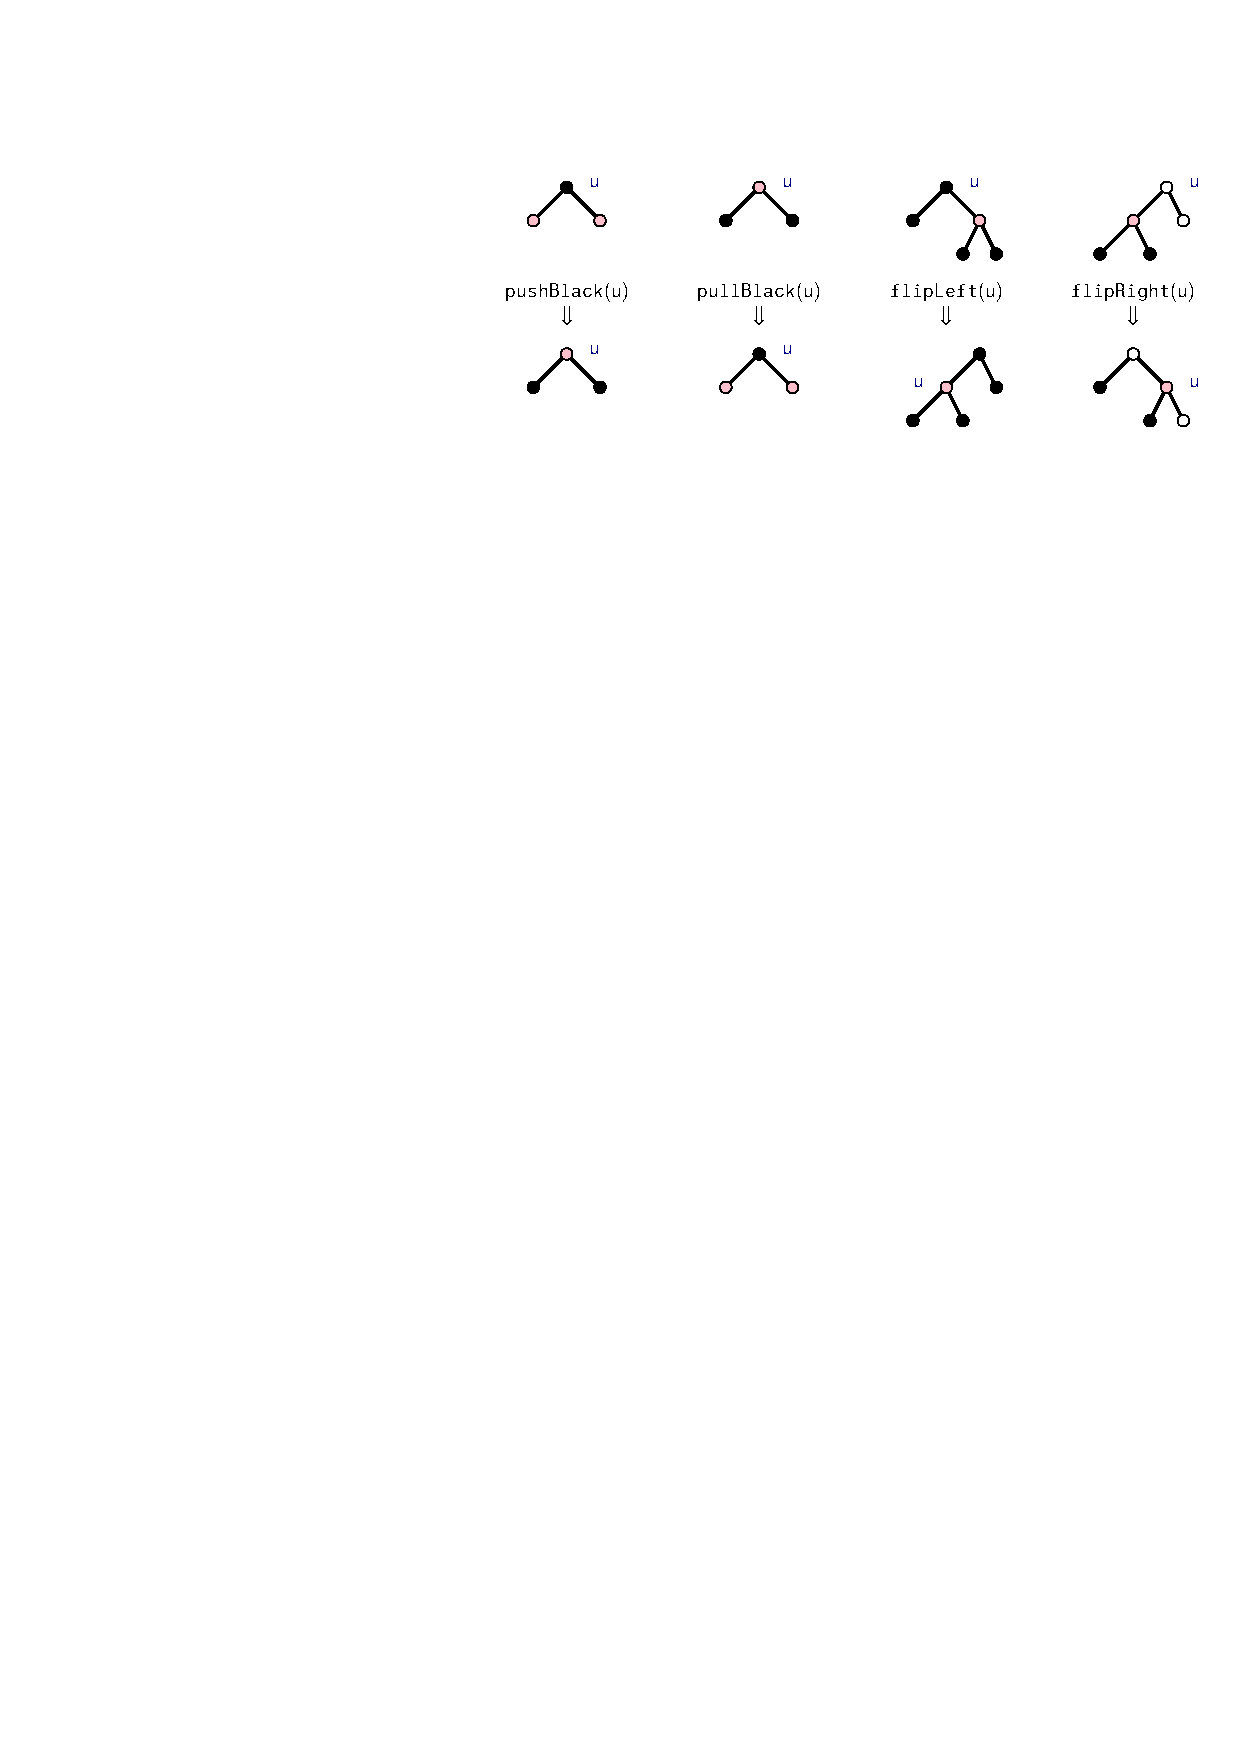
\includegraphics[width=\ScaleIfNeeded]{figs/flippullpush}
  \end{center}
  \caption{Flips, pulls and pushes}
  \figlabel{redblack-flippullpush}
\end{figure}

The #flipLeft(u)# method swaps the colours of #u# and #u.right#
and then performs a left rotation at #u#.  This method reverses the
colours of these two nodes as well as their parent-child relationship:
\codeimport{ods/RedBlackTree.flipLeft(u)}
The #flipLeft(u)# operation
is especially useful in restoring the left-leaning property at a node
#u# that violates it (because #u.left# is black and #u.right# is red).
In this special case, we can be assured that this operation preserves both
the black-height and no-red-edge properties.  The #flipRight(u)# operation
is symmetric with #flipLeft(u)#, when the roles of left and right are reversed.
\codeimport{ods/RedBlackTree.flipRight(u)}

\subsection{Addition}

To implement #add(x)# in a #RedBlackTree#, we perform a standard
#BinarySearchTree# insertion to add a new leaf, #u#, with $#u.x#=#x#$ and
set $#u.colour#=#red#$.  Note that this does not change the black height
of any node, so it does not violate the black-height property.  It may,
however, violate the left-leaning property (if #u# is the right child of
its parent), and it may violate the no-red-edge property (if #u#'s parent
is #red#).  To restore these properties, we call the method #addFixup(u)#.
\codeimport{ods/RedBlackTree.add(x)}

Illustrated in \figref{rb-addfix}, the #addFixup(u)# method takes
as input a node #u# whose colour is red and which may violate the
no-red-edge property and/or the left-leaning property.  The following
discussion is probably impossible to follow without referring to
\figref{rb-addfix} or recreating it on a piece of paper.  Indeed, the
reader may wish to study this figure before continuing.

\begin{figure}
  \begin{center}
    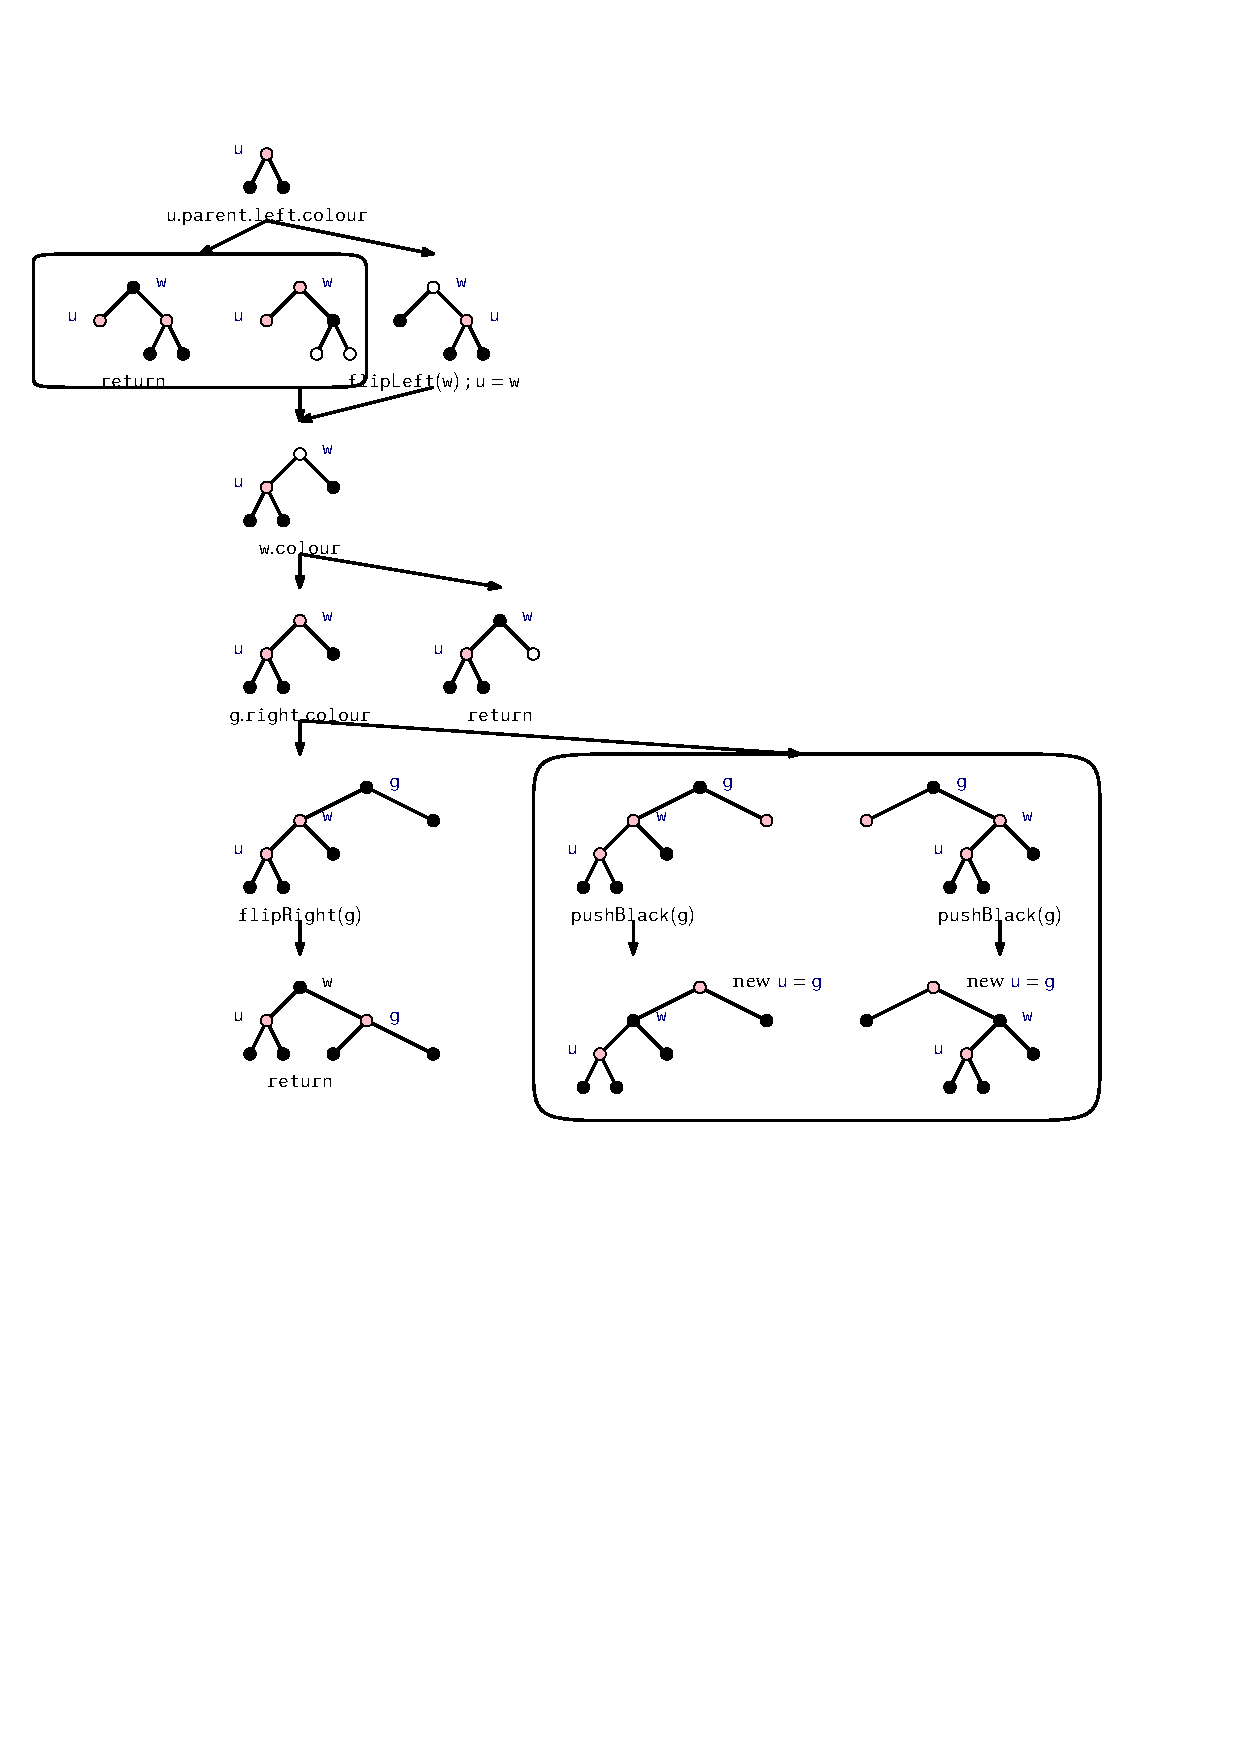
\includegraphics[width=\ScaleIfNeeded]{figs/rb-addfix}
  \end{center}
  \caption{A single round in the process of fixing Property~2 after
  an insertion.}
  \figlabel{rb-addfix}
\end{figure}

If #u# is the root of the tree, then we can colour #u# black to restore
both properties.  If #u#'s sibling is also red, then #u#'s parent must be
black, so both the left-leaning and no-red-edge properties already hold.

Otherwise, we first determine if #u#'s parent, #w#, violates the
left-leaning property and, if so, perform a #flipLeft(w)# operation and
set $#u#=#w#$.  This leaves us in a well-defined state:  #u# is the left
child of its parent, #w#, so #w# now satisfies the left-leaning property.
All that remains is to ensure the no-red-edge property at #u#.  We only
have to worry about the case in which #w# is red, since otherwise #u#
already satisfies the no-red-edge property.

Since we are not done yet, #u# is red and #w# is red.  The no-red-edge
property (which is only violated by #u# and not by #w#) implies that
#u#'s grandparent #g# exists and is black.  If #g#'s right child is red,
then the left-leaning property ensures that both #g#'s children are red,
and a call to #pushBlack(g)# makes #g# red and #w# black.  This restores
the no-red-edge property at #u#, but may cause it to be violated at #g#,
so the whole process starts over with $#u#=#g#$.

If #g#'s right child is black, then a call to #flipRight(g)# makes
#w# the (black) parent of #g# and gives #w# two red children, #u# and
#g#. This ensures that #u# satisfies the no-red-edge property and #g#
satisfies the left-leaning property.  In this case we can stop.
\codeimport{ods/RedBlackTree.addFixup(u)}

The #insertFixup(u)# method takes constant time per iteration and each
iteration either finishes or moves #u# closer to the root.  Therefore,
the #insertFixup(u)# method finishes after $O(\log #n#)$ iterations in
$O(\log #n#)$ time.

\subsection{Removal}

The #remove(x)# operation in a #RedBlackTree# is the most complicated
to implement, and this is true of all known red-black tree variants.
Just like the #remove(x)# operation in a \texttt{BinarySearchTree},
this operation boils down to finding a node #w# with only one child,
#u#, and splicing #w# out of the tree by having #w.parent# adopt #u#.

The problem with this is that, if #w# is black, then the black-height
property will now be violated at #w.parent#.  We may avoid this problem,
temporarily, by adding #w.colour# to #u.colour#.  Of course, this introduces
two other problems:  (1)~if #u# and #w# both started out black, then
$#u.colour#+#w.colour#=2$ (double black), which is an invalid colour.
If #w# was red, then it is replaced by a black node #u#, which may
violate the left-leaning property at $#u.parent#$.  Both of these
problems can be resolved with a call to the #removeFixup(u)# method.
\codeimport{ods/RedBlackTree.remove(x)}

The #removeFixup(u)# method takes as its input a node #u# whose colour is black
(1) or double-black (2).  If #u# is double-black, then #removeFixup(u)#
performs a series of rotations and recolouring operations that move the
double-black node up the tree until it can be eliminated.  During this
process, the node #u# changes until, at the end of this process, #u#
refers to the root of the subtree that has been changed.  The root of
this subtree may have changed colour.  In particular, it may have gone
from red to black, so the #removeFixup(u)# method finishes by checking
if #u#'s parent violates the left-leaning property and, if so, fixing it.
\codeimport{ods/RedBlackTree.removeFixup(u)}

The #removeFixup(u)# method is illustrated in \figref{rb-removefix}.
Again, the following text will be difficult, if not impossible, to follow
without referring to \figref{rb-removefix}.  Each iteration of the loop
in #removeFixup(u)# processes the double-black node #u#, based on one
of four cases:

\begin{figure}
  \begin{center}
    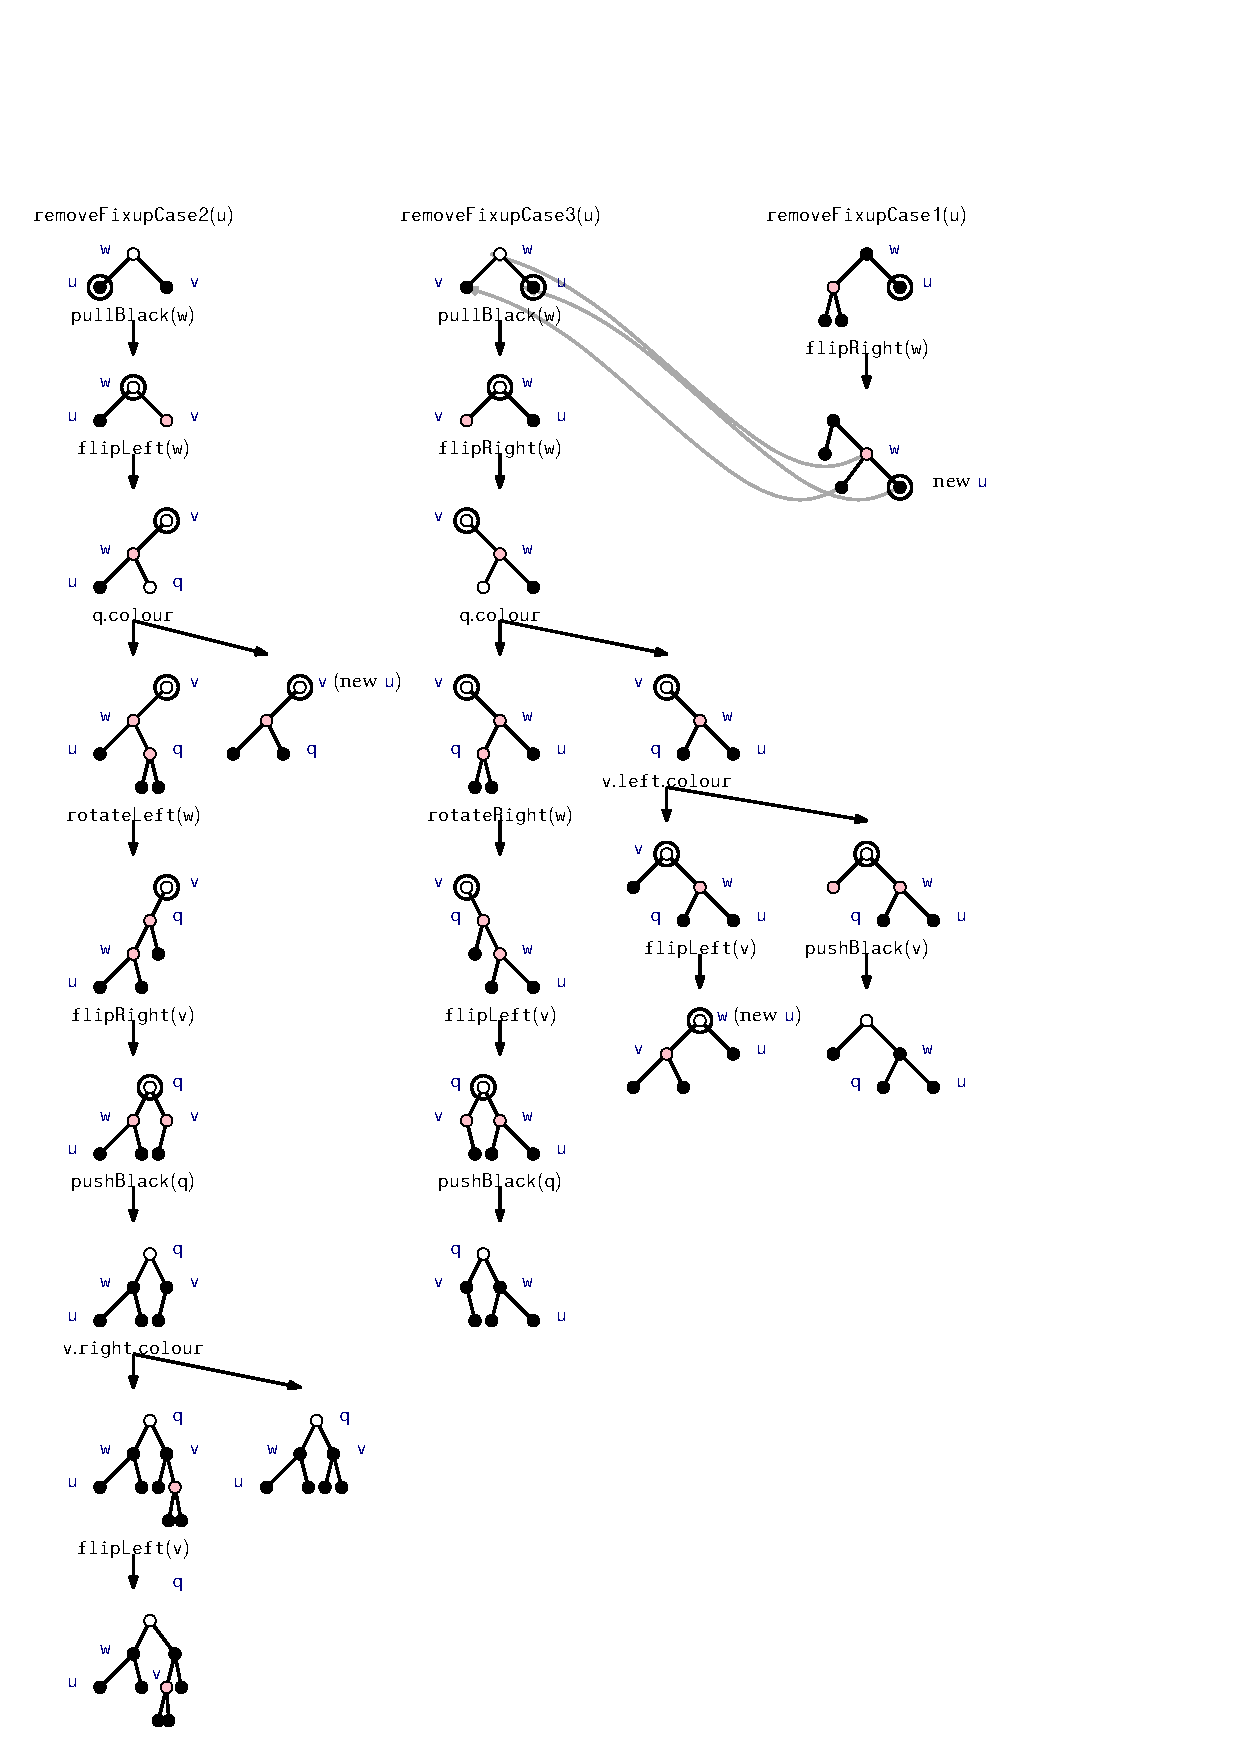
\includegraphics[height=\HeightScaleIfNeeded]{figs/rb-removefix}
  \end{center}
  \caption{A single round in the process of eliminating a double-black node
   after a removal.}
  \figlabel{rb-removefix}
\end{figure}

\noindent
Case 0: #u# is the root.  This is the easiest case to treat.  We recolour
#u# to be black (this does not violate any of the red-black tree
properties).

\noindent 
Case 1: #u#'s sibling, #v#, is red.  In this case, #u#'s sibling is the
left child of its parent, #w# (by the left-leaning property).  We perform
a right-flip at #w# and then proceed to the next iteration.  Note that
this action causes #w#'s parent to violate the left-leaning property and
the depth of #u# to increase.  However, it also implies that the next
iteration will be in Case~3 with #w# coloured red.  When examining Case~3
below, we will see that the process will stop during the next iteration.
\codeimport{ods/RedBlackTree.removeFixupCase1(u)}

\noindent
Case 2: #u#'s sibling, #v#, is black, and #u# is the left child of its
parent, #w#.  In this case, we call #pullBlack(w)#, making #u# black,
#v# red, and darkening the colour of #w# to black or double-black.
At this point, #w# does not satisfy the left-leaning property, so we
call #flipLeft(w)# to fix this.

At this point, #w# is red and #v# is the root of the subtree with which
we started.  We need to check if #w# causes the no-red-edge property to
be violated.  We do this by inspecting #w#'s right child, #q#.  If #q#
is black, then #w# satisfies the no-red-edge property and we can continue
the next iteration with $#u#=#v#$.

Otherwise (#q# is red), so both the no-red-edge property and the left-leaning
properties are violated at #q# and #w#, respectively.  The left-leaning
property is restored with a call to  
#rotateLeft(w)#, but the no-red-edge
property is still violated.  At this point, #q# is the left child of
#v#, #w# is the left child of #q#, #q# and #w# are both red, and #v#
is black or double-black.  A #flipRight(v)#  makes #q# the parent of
both #v# and #w#.  Following this up by a #pushBlack(q)# makes both #v#
and #w# black and sets the colour of #q# back to the original colour of #w#.

At this point, the double-black node is has been eliminated and the
no-red-edge and black-height properties are reestablished.  Only one possible problem remains: the right child of #v# may be red, in which
case the left-leaning property would be violated.  We check this and
perform a #flipLeft(v)# to correct it if necessary.
\codeimport{ods/RedBlackTree.removeFixupCase2(u)}

\noindent
Case 3: #u#'s sibling is black and #u# is the right child of its parent,
#w#.  This case is symmetric to Case~2 and is handled mostly the same way.
The only differences come from the fact that the left-leaning property
is asymmetric, so it requires different handling.

As before, we begin with a call to #pullBlack(w)#, which makes #v# red
and #u# black.  A call to #flipRight(w)# promotes #v# to the root of
the subtree.  At this point #w# is red, and the code branches two ways
depending on the colour of #w#'s left child, #q#.

If #q# is red, then the code finishes up exactly the same way as Case~2
does, but is even simpler since there is no danger of #v# not
satisfying the left-leaning property.

The more complicated case occurs when #q# is black.  In this case,
we examine the colour of #v#'s left child.  If it is red, then #v# has
two red children and its extra black can be pushed down with a call to
#pushBlack(v)#.  At this point, #v# now has #w#'s original colour, and we
are done.

If #v#'s left child is black, then #v# violates the left-leaning property,
and we restore this with a call to #flipLeft(v)#.  We then return the
node #v# so that the next iteration of #removeFixup(u)# then continues
with $#u#=#v#$.
\codeimport{ods/RedBlackTree.removeFixupCase3(u)}.

Each iteration of #removeFixup(u)# takes constant time.  Cases~2 and 3
either finish or move #u# closer to the root of the tree.  Case~0 (where
#u# is the root) always terminates and Case~1 leads immediately to Case~3,
which also terminates.  Since the height of the tree is at most $2\log
#n#$, we conclude that there are at most $O(\log #n#)$ iterations of
#removeFixup(u)#, so #removeFixup(u)# runs in $O(\log #n#)$ time.


\section{Summary}
\seclabel{redblack-summary}

The following theorem summarizes the performance of the #RedBlackTree# data structure:

\begin{thm}
  A #RedBlackTree# implements the #SSet# interface and
  supports the operations #add(x)#, #remove(x)#, and #find(x)# in $O(\log
  #n#)$ worst-case time per operation.
\end{thm}

Not included in the above theorem is the following extra bonus:

\begin{thm}\thmlabel{redblack-amortized}
  Beginning with an empty #RedBlackTree#, any sequence of $m$
  #add(x)# and #remove(x)# operations results in a total of $O(m)$
  time spent during all calls #addFixup(u)# and #removeFixup(u)#. 
\end{thm}

We only sketch a proof of \thmref{redblack-amortized}. By comparing
#addFixup(u)# and #removeFixup(u)# with the algorithms for adding or
removing a leaf in a 2-4 tree, we can convince ourselves that this
property is inherited from a 2-4 tree.  In particular, if we can show
that the total time spent splitting, merging, and borrowing in a 2-4
tree is $O(m)$, then this implies \thmref{redblack-amortized}.

The proof of this theorem for 2-4 trees uses the potential
method
\index{potential method}%
of amortized analysis.\footnote{See the proofs of
\lemref{dualarraydeque-amortized} and \lemref{selist-amortized} for
other applications of the potential method.} Define the potential of an
internal node #u# in a 2-4 tree as
\[
  \Phi(#u#) = 
    \begin{cases} 
      1 & \text{if #u# has 2 children} \\ 
      0 & \text{if #u# has 3 children} \\ 
      3 & \text{if #u# has 4 children}  
    \end{cases}
\]
and the potential of a 2-4 tree as the sum of the potentials of its nodes.
When a split occurs, it is because a node with four children becomes
two nodes, with two and three children.  This means that the overall
potential drops by $3-1-0 = 2$. When a merge occurs, two nodes that used
to have two children are replaced by one node with three children. The
result is a drop in potential of $2-0=2$.  Therefore, for every split
or merge, the potential decreases by two.

Next notice that, if we ignore splitting and merging of nodes, there are
only a constant number of nodes whose number of children is changed by
the addition or removal of a leaf.  When adding a node, one node has
its number of children increase by one, increasing the potential by
at most three.  During the removal of a leaf, one node has its number
of children decrease by one, increasing the potential by at most one,
and two nodes may be involved in a borrowing operation, increasing their
total potential by at most one.

To summarize, each merge and split causes the potential to drop by
at least two.  Ignoring merging and splitting, each addition or removal
causes the potential to rise by at most three, and the potential is always
non-negative.  Therefore, the number of splits and merges caused by $m$
additions or removals on an initially empty tree is at most $3m/2$.
\thmref{redblack-amortized} is a consequence of this analysis and the
correspondence between 2-4 trees and red-black trees.

\section{Discussion and Exercises}

Red-black trees were first introduced by Guibas and Sedgewick \cite{gs78}.
Despite their high implementation complexity they are found in some of
the most commonly used libraries and applications.  Most algorithms and
data structures textbooks discuss some variant of red-black trees.

Andersson \cite{a93} describes a left-leaning version of balanced trees
that is similar to red-black trees but has the additional constraint
that any node has at most one red child.  This implies that these trees
simulate 2-3 trees rather than 2-4 trees.  They are significantly simpler,
though, than the #RedBlackTree# structure presented in this chapter.

Sedgewick \cite{s08} describes two versions of left-leaning red-black
trees.  These use recursion along with a simulation of top-down splitting
and merging in 2-4 trees. The combination of these two techniques makes
for particularly short and elegant code.

A related, and older, data structure is the \emph{AVL tree} \cite{avl62}.
\index{AVL tree}%
AVL trees are \emph{height-balanced}:
\index{height-balanced}%
\index{binary search tree!height balanced}%
At each node $u$, the height
of the subtree rooted at #u.left# and the subtree rooted at #u.right#
differ by at most one.  It follows immediately that, if $F(h)$ is the
minimum number of leaves in a tree of height $h$, then $F(h)$ obeys the
Fibonacci recurrence
\[
   F(h) = F(h-1) + F(h-2)
\]
with base cases $F(0)=1$ and $F(1)=1$.  This means $F(h)$ is approximately
$\varphi^h/\sqrt{5}$, where $\varphi=(1+\sqrt{5})/2\approx1.61803399$ is the
\emph{golden ratio}.  (More precisely, $|\varphi^h/\sqrt{5} - F(h)|\le 1/2$.)
Arguing as in the proof of \lemref{twofour-height}, this implies
\[
   h \le \log_\varphi #n# \approx 1.440420088\log #n# \enspace ,
\]
so AVL trees have smaller height than red-black trees.  The height
balancing can be maintained during #add(x)# and #remove(x)# operations
by walking back up the path to the root and performing a rebalancing
operation at each node #u# where the height of #u#'s left and right
subtrees differ by two.  See \figref{avl-rebalance}.

\begin{figure}
  \begin{center}
    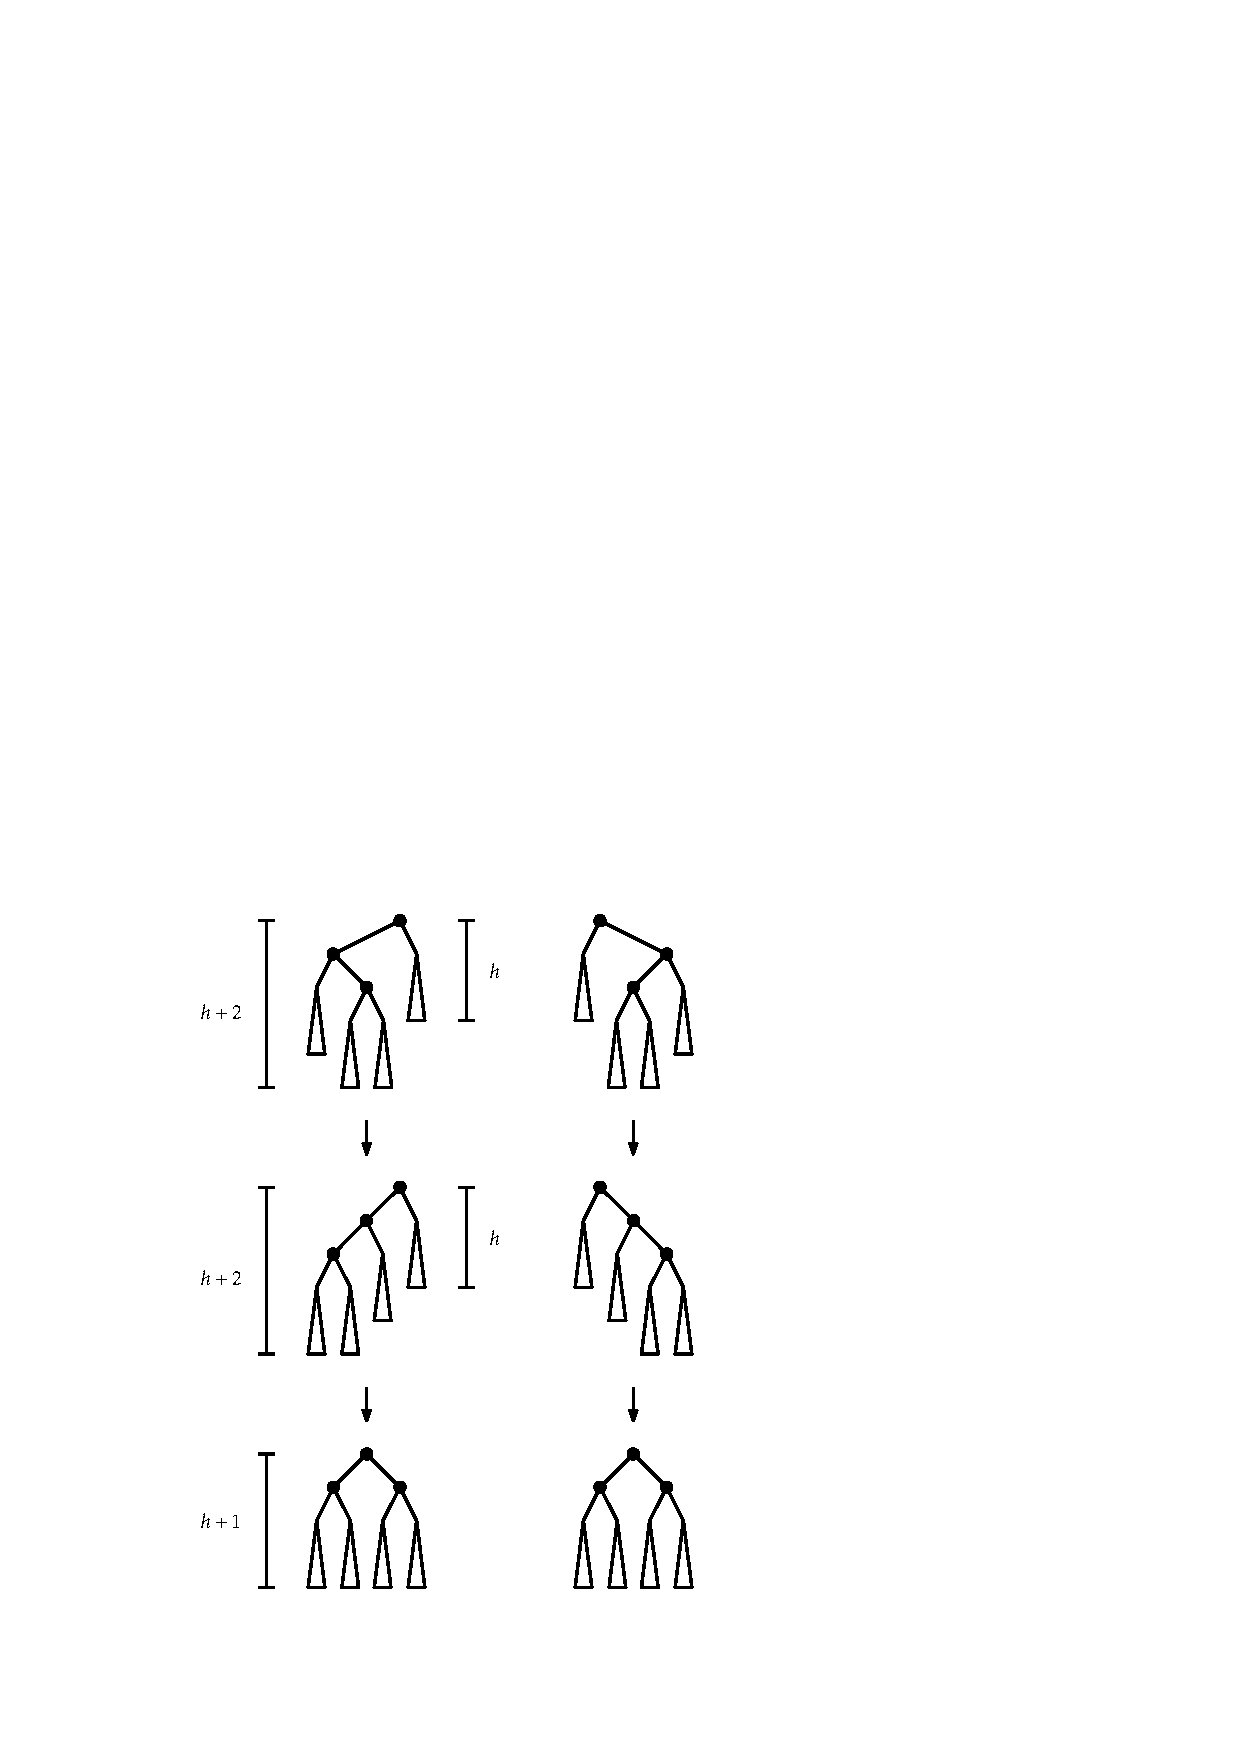
\includegraphics[scale=0.90909]{figs/avl-rebalance}
  \end{center}
  \caption{Rebalancing in an AVL tree.  At most two rotations are required
  to convert a node whose subtrees have a height of $h$ and $h+2$ into a node
  whose subtrees each have a height of at most $h+1$.}
  \figlabel{avl-rebalance}
\end{figure}

Andersson's variant of red-black trees, Sedgewick's variant of red-black
trees, and AVL trees are all simpler to implement than the #RedBlackTree#
structure defined here.  Unfortunately, none of them can guarantee that
the amortized time spent rebalancing is $O(1)$ per update.  In particular,
there is no analogue of \thmref{redblack-amortized} for those structures.

\begin{figure}
  \centering{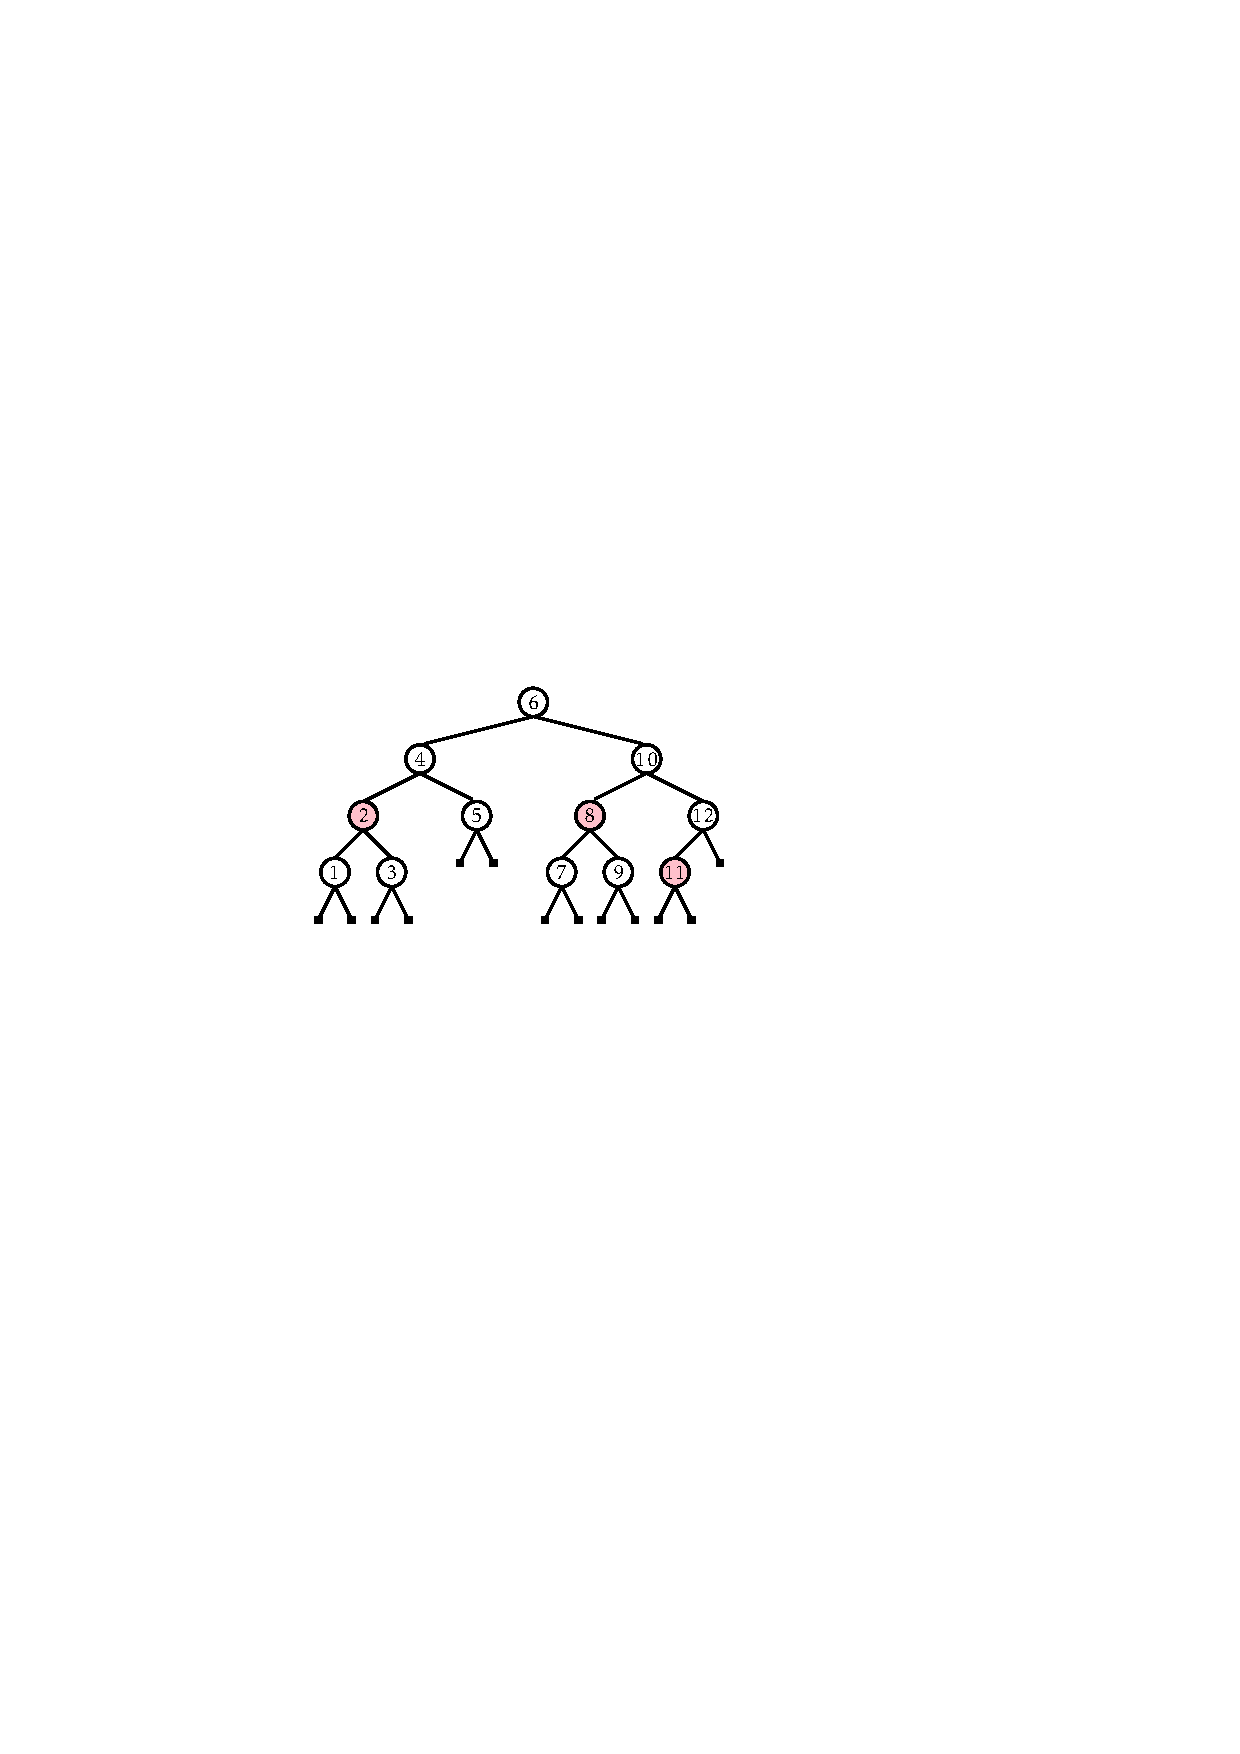
\includegraphics[scale=0.90909]{figs/redblack-example}}
  \caption{A red-black tree on which to practice.}
  \figlabel{redblack-example2}
\end{figure}

\begin{exc}
  Illustrate the 2-4 tree that corresponds to the #RedBlackTree# in
  \figref{redblack-example2}.
\end{exc}

\begin{exc}
  Illustrate the addition of 13, then 3.5, then 3.3 on the #RedBlackTree#
  in \figref{redblack-example2}.
\end{exc}

\begin{exc}
  Illustrate the removal of 11, then 9, then 5 on the #RedBlackTree# in 
  \figref{redblack-example2}.
\end{exc}

\begin{exc}
  Show that, for arbitrarily large values of #n#, there are red-black
  trees with #n# nodes that have height $2\log #n#-O(1)$.
\end{exc}

\begin{exc}
  Consider the operations #pushBlack(u)# and #pullBlack(u)#.  What do
  these operations do to the underlying 2-4 tree that is being simulated
  by the red-black tree?
\end{exc}

\begin{exc}
  Show that, for arbitrarily large values of #n#, there exist sequences
  of #add(x)# and #remove(x)# operations that lead to red-black trees
  with #n# nodes that have height $2\log #n#-O(1)$.
\end{exc}



\begin{exc}
  Why does the method #remove(x)# in the #RedBlackTree# implementation
  perform the assignment #u.parent=w.parent#?  Shouldn't this already
  be done by the call to #splice(w)#?
\end{exc}

\begin{exc}
  Suppose a 2-4 tree, $T$, has $#n#_\ell$ leaves and $#n#_i$ internal nodes.
  \begin{enumerate}
    \item What is the minimum value of $#n#_i$, as a function of $#n#_\ell$?
    \item What is the maximum value of $#n#_i$, as a function of $#n#_\ell$?
    \item If $T'$ is a red-black tree that represents $T$, then how many red
     nodes does $T'$ have?
  \end{enumerate}
\end{exc}

\begin{exc}
  Suppose you are given a binary search tree with #n# nodes and a
  height of at most $2\log #n#-2$.  Is it always possible to colour the
  nodes red and black so that the tree satisfies the black-height and
  no-red-edge properties?  If so, can it also be made to satisfy the
  left-leaning property?
\end{exc}

\begin{exc}\exclabel{redblack-merge}
  Suppose you have two red-black trees $T_1$ and $T_2$ that have the
  same black height, $h$, and such that the largest key in $T_1$ is smaller
  than the smallest key in $T_2$.  Show how to merge $T_1$ and $T_2$
  into a single red-black tree in $O(h)$ time.
\end{exc}

\begin{exc}
  Extend your solution to \excref{redblack-merge} to the case where the
  two trees $T_1$ and $T_2$ have different black heights, $h_1\neq h_2$.
  The running-time should be $O(\max\{h_1,h_2\})$.
\end{exc}



\begin{exc}
  Prove that, during an #add(x)# operation, an AVL tree must perform
  at most one rebalancing operation (that involves at most two rotations;
  see \figref{avl-rebalance}).  Give an example of an AVL tree and a
  #remove(x)# operation on that tree that requires on the order of $\log
  #n#$ rebalancing operations.
\end{exc}

\begin{exc}
  Implement an #AVLTree# class that implements AVL trees as described
  above.  Compare its performance to that of the #RedBlackTree#
  implementation.   Which implementation has a faster #find(x)# operation?
\end{exc}

\begin{exc}
  Design and implement a series of experiments that compare the relative
  performance of #find(x)#, #add(x)#, and #remove(x)# for the #SSet# implemeentations #SkiplistSSet#,
  #ScapegoatTree#, #Treap#, and #RedBlackTree#.  Be sure to include
  multiple test scenarios, including cases where the data is random,
  already sorted, is removed in random order, is removed in sorted order,
  and so on.
\end{exc}
